\documentclass[10pt]{beamer}

\usetheme[progressbar=frametitle]{m}


\usepackage{booktabs}
\usepackage[scale=2]{ccicons}

\usepackage{pgfplots}
\usepackage{graphicx}
\usepackage[export]{adjustbox}
\usepgfplotslibrary{dateplot}

\definecolor{blue_slides}{RGB}{36,55,59}
\definecolor{gray_slides}{RGB}{236,236,236}
\definecolor{beaver_red}{RGB}{161,5,13}
\setbeamercolor{block title}{fg=white,bg=blue_slides}
\setbeamercolor{block body}{fg=black,bg=gray_slides}
\setbeamertemplate{blocks}[rounded][shadow=true]

\title{Smart Grid Survey}
\subtitle{}
\small{\date{\today}}
\author{Marco Amoruso, Daniele Anello, Francesco Farina, Iolanda Rinaldi}
\institute{Università degli Studi di Salerno}
\titlegraphic{\hfill
\includegraphics[scale=0.4]{imgs/logo.png}}

\begin{document}

\maketitle

\begin{frame}
  \frametitle{Table of Contents}
  \setbeamertemplate{section in toc}[sections numbered]
  \tableofcontents[hideallsubsections]
\end{frame}


\section{Smart Grid: \newline panorama attuale e definizione}
\begin{frame}{Rete elettrica attuale}
	\begin{figure}[h] 
		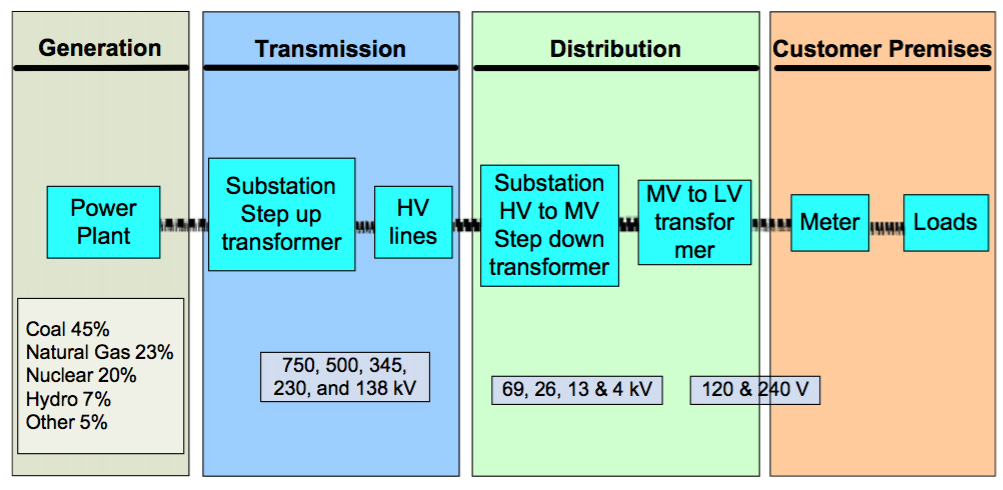
\includegraphics[scale=0.25]{imgs/elect_grid.png}
		%\caption{Rete elettrica attuale}
	\end{figure}

\begin{itemize}[<+- | alert@+>]
	\item Tre sottosistemi distinti
		\begin{itemize}
		\item Generazione
		\item Trasmissione
		\item Distribuzione
		\end{itemize}
\end{itemize}
\end{frame}

\begin{frame}{Rete elettrica attuale}
	\begin{itemize}[<+- | alert@+>]
	\item Comunicazione unidirezionale
	\item Interconnessione e ridondanza per risolvere i problemi
	\item Distribuzione dell'energia gestita da un controllore centralizzato
	\end{itemize}

\end{frame}

\begin{frame}{Problemi della rete elettrica attuale}
	\begin{itemize}[<+- | alert@+>]
	\item Numerosi problemi da risolvere
		\begin{itemize}
		\item Diversificazione della generazione di energia
		\item Gestione delle richieste utente
		\item Conservazione dell’energia
		\item Riduzione globale dell’emissione di anidride carbonica
		\end{itemize}
	\item Non ci si può affidare all'infrastruttura attuale
		\begin{itemize}
			\item Inadeguatezza della struttura gerarchica
			 	\begin{itemize}
			 	\item Effetto domino in caso di guasti
			 	\end{itemize}
		\end{itemize}
	\end{itemize}
\end{frame}

\begin{frame}{Problemi della rete elettrica attuale}
	\begin{itemize}[<+- | alert@+>]
	\item Necessità di digitalizzare le infrastrutture critiche
		\begin{itemize}
		\item Aggiunta di capacità di computazione e comunicazione
		\item Requisito necessario per gestire l'ambiente che muta
		\end{itemize}
	\item Esempio di digitalizzazione: meter analogico $\rightarrow$ Smart meter
		\begin{itemize}
			\item Dispositivo disconnesso e non critico $\rightarrow$ Dispositivo connesso ad Internet che può generare dati critici
		\end{itemize}
\item Fondamentale la sicurezza dei dati e dei comandi degli smart meter
\item Obiettivo della survey: capire la sicurezza della nuova infrastruttura
	\end{itemize}
\end{frame}

\begin{frame}{Perché la Smart Grid?}
	\begin{itemize}[<+- | alert@+>]
	\item Vari fattori influenzano lo sviluppo della rete elettrica
	 \begin{itemize}
	  	\item Strutture non più adeguate
	  	\item Vincoli termici e operativi
	  	\item Sicurezza delle forniture
	  	\item Iniziative nazionali
	 \end{itemize}
	\item Significative opportunità offerte da 
	\begin{itemize}
	\item ICT
	\item Monitoraggio costante delle componenti della rete
	\end{itemize}
	\end{itemize}
\end{frame}


\begin{frame}{Perché la Smart Grid?}
	\begin{figure}[h] 
		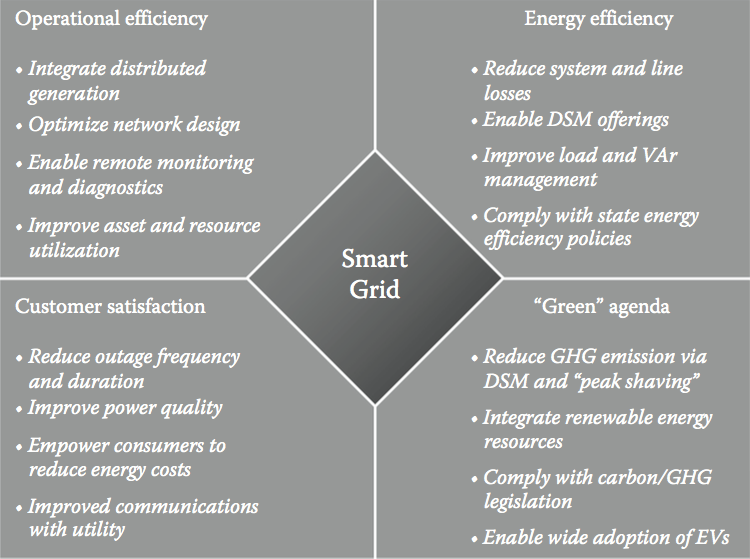
\includegraphics[scale=0.25]{imgs/benefits.png}
		%\caption{Vantaggi introdotti dalla Smart Grid}
	\end{figure}
\end{frame}


\begin{frame}{Smart Grid: definizione}
\begin{itemize}[<+- | alert@+>]
\item Smart Grid = tecnologie + soluzioni per utenti finali
\item Non esiste una singola definizione precisa
\item È possibile trovare una serie di caratterizzazioni
\end{itemize}
\end{frame}

\begin{frame}{Smart Grid: definizione}
\begin{block}{Secondo l’European Technology Platform}
\begin{quote}
\textit{``Una Smart Grid è una rete elettrica che può integrare intelligentemente le azioni di tutti gli utenti connessi ad essa - generatori, consumatori - in modo da fornire efficientemente un’alimentazione elettrica che sia sostenibile, economica e sicura.”}
\end{quote}
\end{block}
\end{frame}

\begin{frame}{Smart Grid: definizione}
\begin{block}{In accordo all’US Department of Energy}
\begin{quote}
\textit{``Una Smart Grid utilizza la tecnologia digitale per migliorare l’affidabilità, la sicurezza e l’efficienza (sia economica che energetica) del sistema elettrico, a partire dalla generazione su larga scala, attraverso il sistema di distribuzione, fino ai consumatori, ed attraverso un numero crescente di risorse di storage e di generazione distribuita.”}
\end{quote}
\end{block}
\end{frame}


\begin{frame}{Smart Grid: definizione}
\begin{block}{Per \textit{Smarter Grids: The Opportunity}}
\begin{quote}
\textit{``Una Smart Grid utilizza sensing, embedded processing e comunicazioni digitali per far sì che la rete elettrica sia osservabile (capace di essere misurata e visualizzata), controllabile (capace di essere manipolata ed utilizzata), automatizzata (capace di adattarsi ed autoripararsi), pienamente integrata (pienamente interoperabile con sistemi esistenti e con la capcità di incorporare un insieme di diverse sorgenti energetiche).”}
\end{quote}
\end{block}
\end{frame}


\begin{frame}{Requisiti di una Smart Grid}
\begin{itemize}[<+- | alert@+>]
\item Quality of Service
	\begin{itemize}
		\item Bassa latenza: la maggior parte delle interazioni deve avvenire in tempo reale
		\item Larghezza di banda sufficiente per permettere la trasmissione simultanea di messaggi senza impatto sulla latenza
	\end{itemize}
\item Interoperabilità
	\begin{itemize}
		\item Abilità delle diverse parti della Smart Grid di lavorare insieme
	\end{itemize}
\end{itemize}
\end{frame}

\begin{frame}{Requisiti di una Smart Grid}
\begin{itemize}[<+- | alert@+>]
\item Scalabilità
	\begin{itemize}
		\item Facilitare l’inserimento di nuovi dispositivi, nuovi servizi, e meccanismi di monitoraggio real-time
	\end{itemize}
\item Standardizzazione
	\begin{itemize}
		\item IEEE P2030 group si occupa di definire standard e linee guida
	\end{itemize}
\end{itemize}
\end{frame}

\begin{frame}{Requisiti di una Smart Grid}
\begin{itemize}[<+- | alert@+>]
\item Sicurezza
	\begin{itemize}
		\item Gestire attacchi volontari (terrorismo, spionaggio, utenti non contenti)
		\item Gestire manomissioni involontarie (fallimenti delle attrezzature, disastri naturali)
		\item North American Electrical Reliability Corporation-Critical Infrastructure Protection (NERC-CIP), IEEE, National Infrastructure Protection Plan (NIPP), e NIST stabiliscono i requisiti di sicurezza della Smart Grid
		\item Denominatore comune: autenticazione, autorizzazione e tecnologie per la privacy
	\end{itemize}
\end{itemize}
\end{frame}


\begin{frame}{Building Blocks: requisiti}
\begin{itemize}[<+- | alert@+>]
\item Building blocks rete elettrica $\rightarrow$ Smart Grid
\begin{itemize}
	\item Monitoraggio/sensing
	\item Comunicazione
	\item Controllo
\end{itemize}
\item Requisiti
\begin{itemize}
\item Rilevare malfunzionamenti/deviazioni dal normale range operativo
\item Permettere che l’input dei sensori raggiunga gli elementi di controllo
\item Generare messaggi per assicurarsi che la trasmissione sia conforme alle aspettative
\end{itemize}
\end{itemize}
\end{frame}


\section{Architettura}
\begin{frame}[fragile]{Architettura}
	\begin{figure}[h] 
		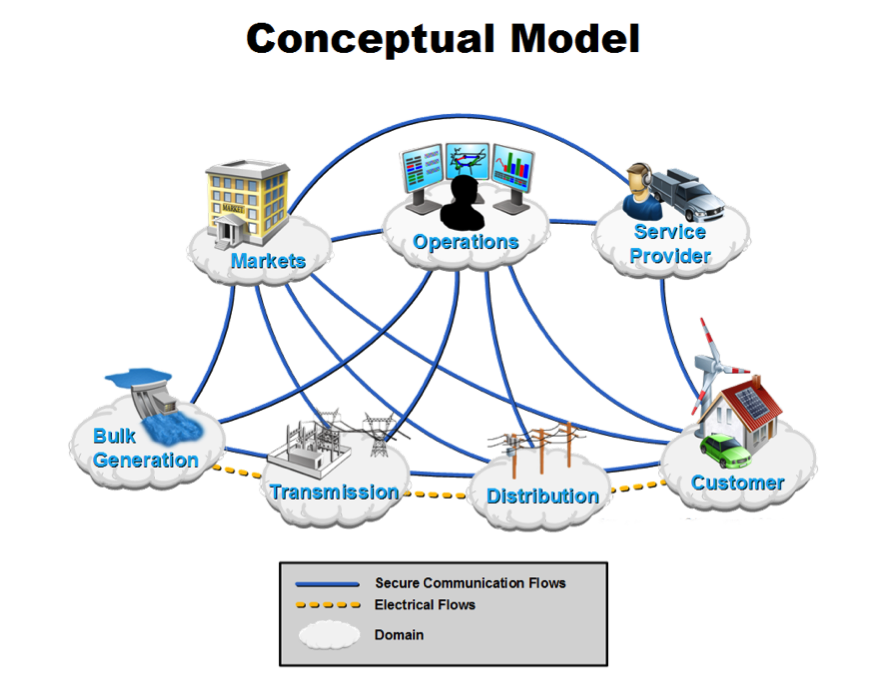
\includegraphics[scale=0.6]{imgs/sg.png}
	\end{figure}
\end{frame}

% Energy and supporting ancillary services (capacity that can be dispatched when needed) are procured through the Markets domain, scheduled and operated from the Operations domain, and finally delivered through the Transmission domain to the distribution system and finally to the Customer domain.

\begin{frame}[fragile]{Architettura}
	\vspace{-10pt}
	\begin{figure}[h] 
		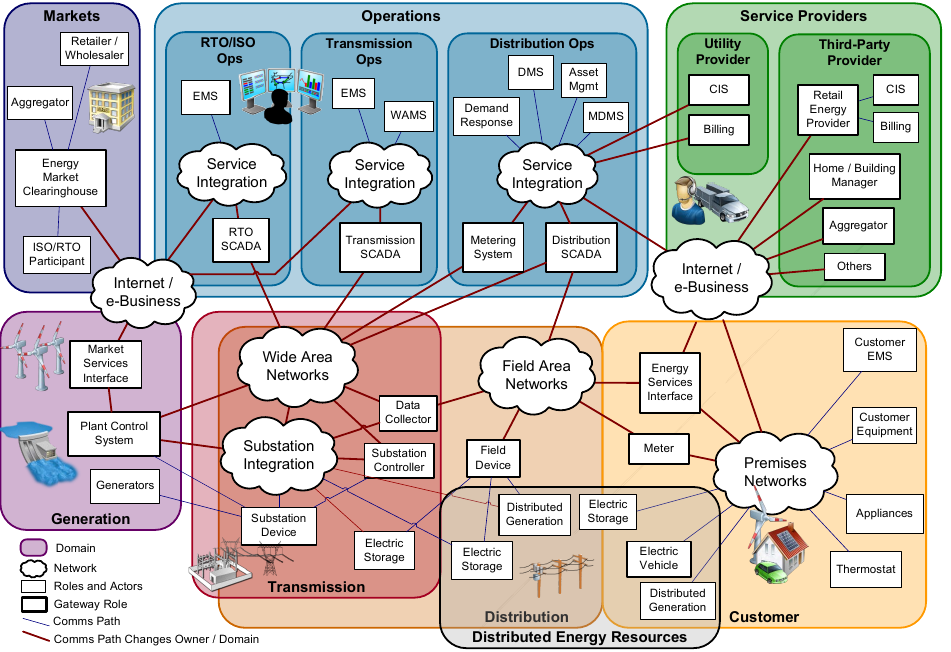
\includegraphics[scale=0.45]{imgs/arch.png}
	\end{figure}
\end{frame}

%\begin{frame}[fragile]
%  \frametitle{Smart Grid Framework}
%	\begin{figure}[h] 
%		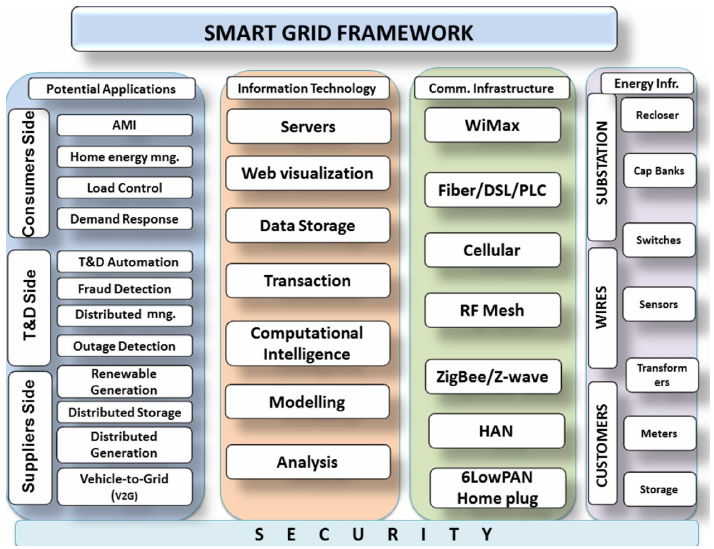
\includegraphics[scale=0.6]{imgs/sgframework.png}
%	\end{figure}
%\end{frame}

%%% CUSTOMER %%% 

\begin{frame}[fragile]{Customer} 
	\begin{figure}[h] 
		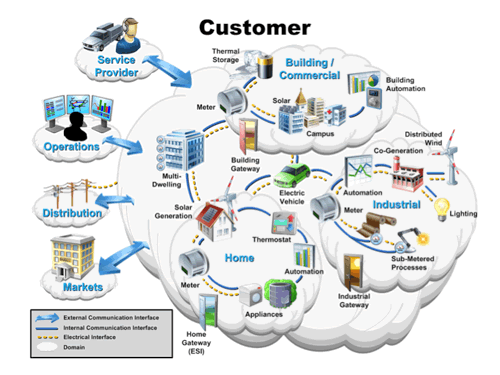
\includegraphics[scale=0.45]{imgs/cust.png}
	\end{figure}
\end{frame}

\begin{frame}[fragile]{Customer} 
		\begin{block}{Smart meter}
		 E' un dispositivo elettronico che registra consumi di energia elettrica
		\begin{itemize}
			\item Comunica informazioni per scopi di fatturazione
			\item Blocca la fornitura di energia  % bad pay o demande response
			\item Notifica informazioni per monitoraggio e in caso di manomissione % comunica con i display   
		\end{itemize}
		\end{block}
		\pause
		\begin{block}{Advanced Metering Infrastructure} % sistema che integra smart meter, display, termostati ecc., reti di comunicazione verso i concentratori di dati e sistemi di gestione dei dati
		\begin{itemize}
			\item Consente una comunicazione bidirezionale fra utility e consumer % ciò consente di inviare comandi per info di pricing basate sul tempo, azioni di domanda risposta o disconnessioni remote
			\item Misura, colleziona, analizza il consumo energetico e comunica con smart device
		\end{itemize}		
		\end{block}	
\end{frame}

%%% MARKETS %%% 

% I mercati sono il luogo in cui le attività di rete vengono acquistate e vendute
% La comunicazione tra il dominio dei mercati e dei domini che forniscono energia sono fondamentali per una efficiente corrispondenza  di produzione con il consumo è dipendente dai mercati. I domini di approvvigionamento energetico sono il dominio di Bulk gen e delle Risorse energetiche distribuite (DER)
% Comunicazioni per le interazioni di dominio dei mercati devono essere affidabili. Essi devono essere tracciabili e verificabili.
\begin{frame}[fragile]{Markets}
	\begin{figure}[h] 
		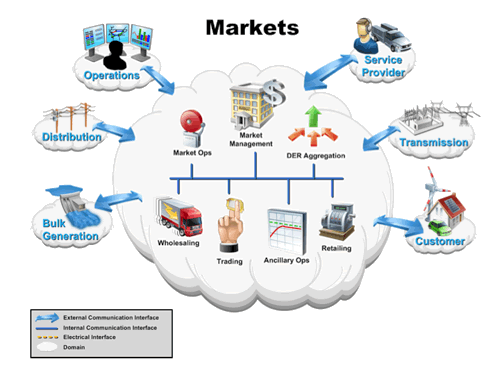
\includegraphics[scale=0.45]{imgs/market.png}
	\end{figure}
\end{frame}

%%% SERVICE PROVIDER %%%

% supporta i processi di business dei produttori del sistema di alimentazione, distributori e clienti
% Questi processi di business vanno da servizi di pubblica utilità tradizionali, come la gestione della fatturazione e conto del cliente, ai servizi avanzati al cliente, come la gestione del consumo energetico e la produzione di energia casalinga.
\begin{frame}[fragile]{Service Provider}
	\begin{figure}[h] 
		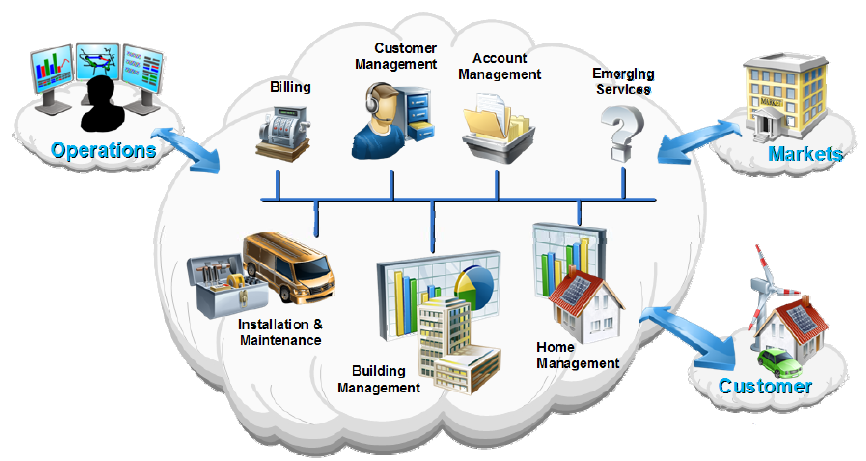
\includegraphics[scale=0.45]{imgs/ser.png}
	\end{figure}
\end{frame}

\begin{frame}[fragile]{Service Provider}
	\begin{itemize}[<+- | alert@+>]
		\item Sviluppano interfacce e standard per un sistema basato su un modello di mercato dinamico, proteggendo le infrastrutture di energia critiche   
		\item Non devono compromettere la sicurezza informatica, l'affidabilità, la stabilità, l'integrità o la sicurezza della rete %quando forniscono servizi esistenti o emergenti
		\item Creano servizi e prodotti per rispondere alle nuove esigenze e le opportunità offerte dall'evoluzione delle Smart Grid 
		\item Rappresentano una zona di notevole nuova crescita economica
	\end{itemize}
\end{frame}



%%% OPERATION %%% 

% responsabile del buon funzionamento del sistema di alimentazione.
\begin{frame}[fragile]{Operations}
	\begin{figure}[h] 
		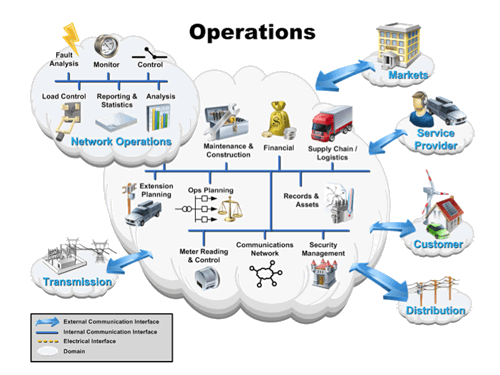
\includegraphics[scale=0.45]{imgs/ope.png}
	\end{figure}
\end{frame}

% Monitoring: supervisionare la topologia della rete, connettività, condizioni di carico, include i dispositivi intelligenti (IED) e dispositivi sul campo, in grado di reportare lo stato della rete

% Control: supervisiona ampie aree, substation, controlli automati o manuali

% Fault Management: migliora la velocità di identificazione di fault, in modo da effetturare ripristino

% Analysis: si confrontano dati in tempo reale e non per ricavare info su incidenti di rete, connettività per scopi di manutenzione

% Operational Planning: mantengono il costo basso della potenza attraverso la generazione di picco, la commutazione, eliminazione del carico o la risposta alla domanda.



%%% GENERATION %%%

% Fornisce energia ai consumers. La generazione di energia è il processo di creazione di energia da diverse fonti energetiche. Tale energia viene portata attraverso il sistema di trasmissione. Comunicazioni con il dominio di trasmissione sono le più critici perché senza trasmissione, i clienti non possono essere serviti.
\begin{frame}[fragile]{Generation}
	\begin{figure}[h] 
		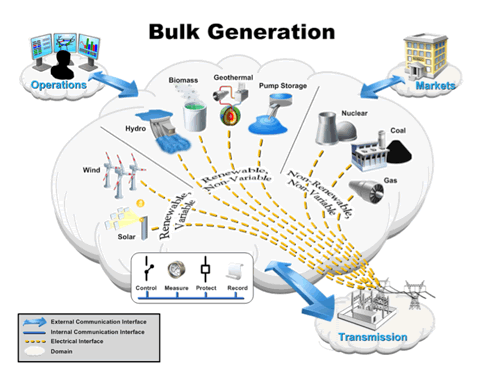
\includegraphics[scale=0.45]{imgs/gen.png}
	\end{figure}
\end{frame}

\begin{frame}[fragile]{Generation}
	\begin{itemize}[<+- | alert@+>]
		\item Gestire il flusso energetico e l'affidabilità del sistema % fasori su substation per modificarne il flusso
		\item Reagire rapidamente ai guasti, interruzioni di corrente o abbassamenti di tensioni % per alta affidabilità
		\item Monitoraggio delle strutture per valutarne le condizioni
		%\item Cruciali risultano comunicazioni in caso di guasti o scarsa fornitura d'energia % energy storage presente su sistemi di trasmissione e distribuzione devono aiutare
	\end{itemize}
\end{frame}


%%% TRASMISSION %%% 

% Trasferimento di massa di energia elettrica da fonti di generazione alla distribuzione attraverso molteplici substation
% include remote terminal units, substation meters, protection relays, power quality monitors, phasor measurement units, sag monitors, fault recorders, e substation user interfaces.
\begin{frame}[fragile]{Transmission}
	\begin{figure}[h] 
		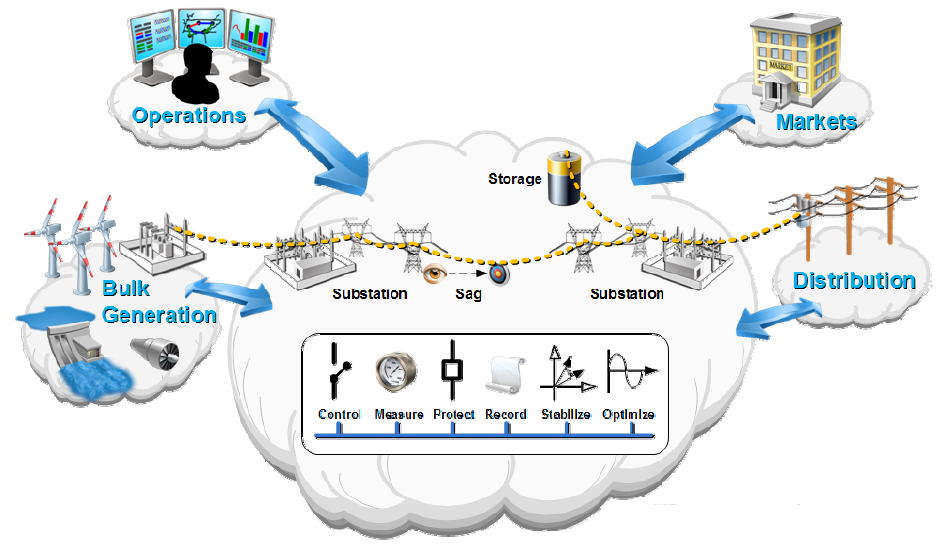
\includegraphics[scale=0.45]{imgs/tras.png}
	\end{figure}
\end{frame}

% rilevatore di abbassamento di linea (sag)
\begin{frame}[fragile]{Transmission}
	\begin{itemize}[<+- | alert@+>]
		\item Gestita da un Regional Transmission Operator o Independent System Operator (RTO/ISO)
			\begin{itemize}
				\item Mantiene la stabilità della rete bilanciando la generazione con la domanda energitica
			\end{itemize}				
		\item Monitorata da sistemi di supervisione e controllo di acquisizione dati
		\item Composta da substation, torri di trasmissione, linee elettriche e dispositivi di telemetria	 
	\end{itemize}
\end{frame}

% Una substation elettrica è un punto di riferimento dei sistemi di generazione, trasmissione e distribuzione, dove il voltaggio viene trasformato da alto a basso e viceversa mediante trasformatori. Ci sono diversi tipi di substation: trasmissione, distribuzione, raccolta, smistamento.
\begin{frame}[fragile]{Transmission}
	\begin{itemize}[<+- | alert@+>]
		\item Le substation sono una componente chiave del sistema di trasmissione
		\begin{itemize}
			\item 
		\end{itemize}
	\end{itemize}
\end{frame}
%%% DISTRIBUTION %%% 

\begin{frame}[fragile]{Distribution}
	\begin{figure}[h] 
		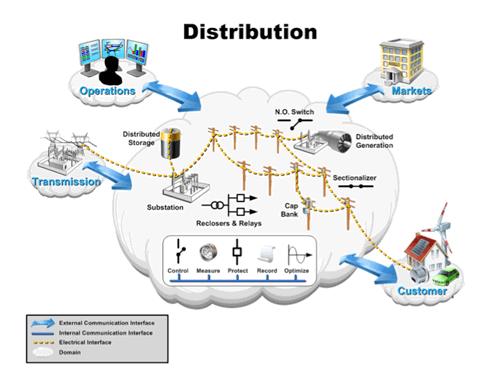
\includegraphics[scale=0.45]{imgs/distr.png}
	\end{figure}
\end{frame}


\section{Smart Grid Cybersecurity}
\begin{frame}{Smart Grid Cybersecurity: Sommario}
\begin{itemize}
\item Stuxnet
\item Definire la sicurezza
	\begin{itemize}
	\item Confidentiality
	\item Integrity
	\item Availability
	\item Control
	\item Authenticity
	\item Usability
	\end{itemize}
\item Building blocks
	\begin{itemize}
		\item Layered security model
		\item Authentication
		\item Authorization
		\item Auditing
		\item Key management
		\item Message, Network and System integrity
	\end{itemize}
\item Threats and impacts
	\begin{itemize}
		\item Consumer threats
		\item Utility companies threats
	\end{itemize}
\end{itemize}
\end{frame}


\begin{frame}{Smart Grid Cybersecurity: Sommario}
\begin{itemize}
\alert<1>{\item Stuxnet}
\item Definire la sicurezza
	\begin{itemize}
	\item Confidentiality
	\item Integrity
	\item Availability
	\item Control
	\item Authenticity
	\item Usability
	\end{itemize}
\item Building blocks
	\begin{itemize}
		\item Layered security model
		\item Authentication
		\item Authorization
		\item Auditing
		\item Key management
		\item Message, Network and System integrity
	\end{itemize}
\item Threats and impacts
	\begin{itemize}
		\item Consumer threats
		\item Utility companies threats
	\end{itemize}
\end{itemize}
\end{frame}
%Definire un worm
%Diffusione inconsapevole
%Data la facile diffusione si pensava a una propagazione su scala mondiale
%Variante Flame: spio e invio dati a blocchi (per non farmi beccare)
\begin{frame}
  \frametitle{Un caso esemplare di attacco: Stuxnet}
  \begin{itemize}[<+- | alert@+>]
  	\item Noto \textbf{\color{blue_slides}worm} di 500 Kbyte scoperto nel 2010 %da VirusBlokAda, una società di sicurezza bielorussa
  	\item Attaccava in 3 fasi:
  	\begin{enumerate}[<+- | alert@+>]
  		\item Attaccava macchine Windows e reti, replicandosi ripetutamente
  		\item Ricercava software Siemens Step7 %Windows-based e utilizzato per programmare sistemi di controllo industriale e infine
  		\item Comprometteva i programmable logic controller
  	\end{enumerate}
  \end{itemize}
  \pause
  \begin{block}{}
  Stuxnet è stato creato dal governo USA in collaborazione col governo Israeliano e diffuso nella centrale iraniana di Natanz
  \end{block}
  \pause
   \begin{block}{Scopo}
   	Sabotare la centrifuga della centrale tramite comandi inviati all’hardware di controllo industriale responsabile della velocità di rotazione delle turbine con l'intento di danneggiarle
   \end{block}
\end{frame}

\begin{frame}{Un caso esemplare di attacco: Stuxnet}
	\begin{figure}[h] 
		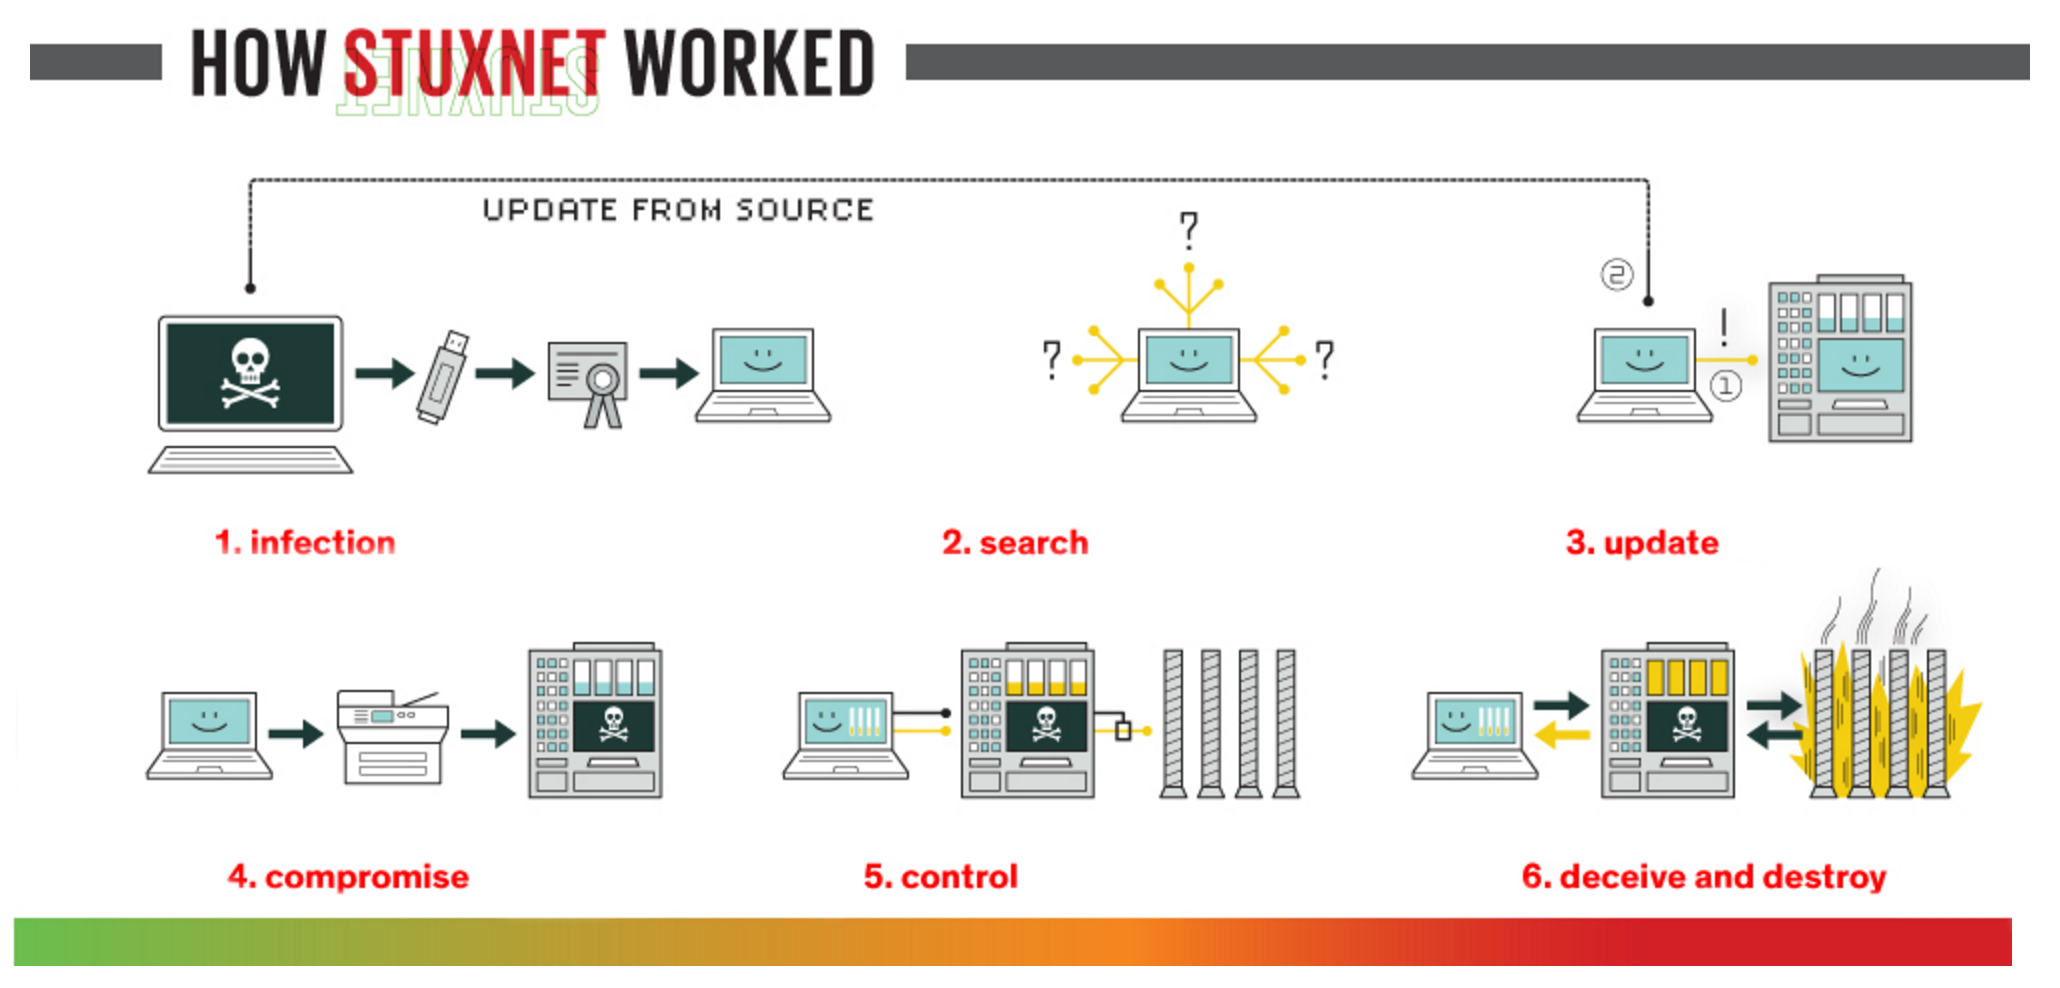
\includegraphics[scale=0.3,cfbox=blue_slides 1pt 0pt]{imgs/stuxnet_hsw.png}
	\end{figure}
\end{frame}
%1. Infection: Entra nel sistema attraverso il collegamento di una penna USB e procede con l’infettare tutte le macchine su cui gira Windows (elude sistemi di automated-detection) (grazie a un certificato digitale che lo fa sembrare affidabile)
%2. Search: Verifica se una macchina è parte del sistema di controllo industriale creato da Siemens
%3. Update: Se il sistema è quello target, il worm accede ad Internet per scaricare una versione più recente di se stesso
%4. Compromise: Compromette i controllori logici del sistema target (sfrutta la vulnerabilità zero-day)
%5. Control: Spia le operazioni del sistema target ed utilizza le informazioni raccolte per prendere il controllo delle centrifughe (portandole al deterioramento)
%6. Deceive & Destroy: Fornisce informazioni fittizie ai controllori assicurandosi che non si accorgeranno del problema

\begin{frame}{Smart Grid Cybersecurity: Sommario}
\begin{itemize}
\item Stuxnet
\alert<1>{\item Definire la sicurezza}
	\begin{itemize}
	\alert<1>{\item Confidentiality}
	\alert<1>{\item Integrity}
	\alert<1>{\item Availability}
	\alert<1>{\item Control}
	\alert<1>{\item Authenticity}
	\alert<1>{\item Usability}
	\end{itemize}
\item Building blocks
	\begin{itemize}
		\item Layered security model
		\item Authentication
		\item Authorization
		\item Auditing
		\item Key management
		\item Message, Network and System integrity
	\end{itemize}
\item Threats and impacts
	\begin{itemize}
		\item Consumer threats
		\item Utility companies threats
	\end{itemize}
\end{itemize}
\end{frame}

\begin{frame}
  \frametitle{Definire la sicurezza: Parkerian hexad}
  	\begin{figure}[h] 
		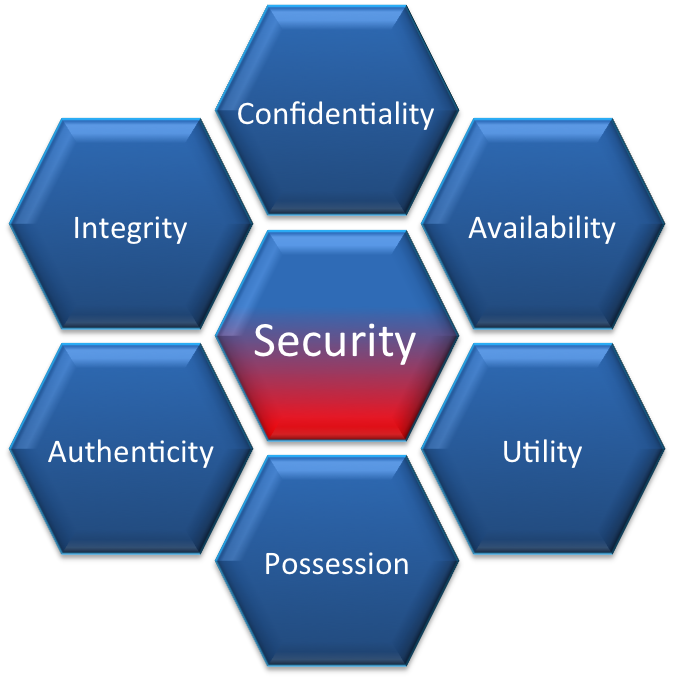
\includegraphics[scale=0.45]{imgs/hexad.png}
		%\caption{Parkerian hexad}
	\end{figure}
\end{frame}

\begin{frame}
  \frametitle{Definire la sicurezza}
  \textbf{Confidentiality}
  	\begin{itemize}[<+- | alert@+>]
  		\item Dati confidenziali $\rightarrow$ se noti, potrebbero causare danni alla sicurezza delle operazioni di tutto il sistema
  		\item Informazioni ricavate dal lavoro delle componenti della Smart Grid
  		\item Dati personali dei clienti $\rightarrow$ garantire la \textit{privacy}
  		\item Informazioni aziendali
  		\item Punti che introducono rischio: locazioni di memoria e meccanismi di trasmissione dati
  		\item Soluzioni: cifratura dei dati e controllo degli accessi
  	\end{itemize}
  %\end{itemize}
\end{frame}

\begin{frame}
  \frametitle{Definire la sicurezza}
   \textbf{Integrity}
  	\begin{itemize}[<+- | alert@+>]
  	\item Abilità del sistema di evitare che le informazioni siano modificate da persone o da sistemi non autorizzati
  	\item Mancanza di integrity $\rightarrow$ il sistema riceve dati non accurati $\rightarrow$ instabilità della Smart Grid
  	\item Punti che introducono rischio: componenti in cui si consente il passaggio dati da un sistema ad un altro
  	\item Soluzioni: \textit{auditing}, \textit{authorization}, \textit{nonrepudiation}, \textit{message-signing}
  	\end{itemize}
\end{frame}

\begin{frame}
  \frametitle{Definire la sicurezza}
   \textbf{Availability}
  	\begin{itemize}[<+- | alert@+>]
  	\item Capacità del sistema di compiere il lavoro che gli è stato assegnato, nel momento in cui se ne ha bisogno 
  	\item Punti che introducono rischio: sistema che gestisce le comunicazioni e l'inoltro di comandi
  	\item Soluzioni: tecniche di ridondanza
  	\end{itemize}
  	\pause
   \textbf{Control (o Possession)}
  	\begin{itemize}[<+- | alert@+>]
  	\item Capacità di controllare le informazioni che necessitano protezione
  	\item Mancanza di controllo dati $\rightarrow$  compromissione del sistema che li trasmette $\rightarrow$ provenienza delle informazioni non garantita $\rightarrow$ diminuzione dell'affidabilità
  	\end{itemize}
\end{frame}

\begin{frame}
  \frametitle{Definire la sicurezza}
   \textbf{Authenticity}
  	\begin{itemize}[<+- | alert@+>]
  	\item Processo utilizzato per descrivere la certezza della provenienza
  	\item Assicurarsi che la fonte dei dati e i dati stessi siano autentici
  	\end{itemize}
  	\pause
  \textbf{Usability (o Utility)}
  \begin{itemize}[<+- | alert@+>]
  \item Assicurare che i dati siano utilizzabili
  \item Flusso di dati cifrato $\rightarrow$ garantisce la sicurezza ma rende difficile far sì che le informazioni siano utili
  \item Usabilità fornisce valore a livello aziendale $\rightarrow$ trattato come il requisito a più alta priorità
  \end{itemize}
\end{frame}

\begin{frame}{Smart Grid Cybersecurity: Sommario}
\begin{itemize}
\item Stuxnet
\item Definire la sicurezza
	\begin{itemize}
	\item Confidentiality
	\item Integrity
	\item Availability
	\item Control
	\item Authenticity
	\item Usability
	\end{itemize}
\alert<1>{\item Building blocks}
	\begin{itemize}
		\alert<1>{\item Layered security model}
		\alert<1>{\item Authentication}
		\alert<1>{\item Authorization}
		\alert<1>{\item Auditing}
		\alert<1>{\item Key management}
		\alert<1>{\item Message, Network and System integrity}
	\end{itemize}
\item Threats and impacts
	\begin{itemize}
		\item Consumer threats
		\item Utility companies threats
	\end{itemize}
\end{itemize}
\end{frame}

\begin{frame}
  \frametitle{Building blocks}
  \textbf{Layered security model}
  \begin{itemize}
  \item Struttura ad anello 
  \item Comunicazione tra gli strati del sistema sicura
%	  \begin{itemize}
%  	\item Uno strato esterno non può avere libero accesso alle risorse presenti su uno strato più interno
%  	\item Le richieste per le risorse non possono saltare gli anelli
%  	\end{itemize}
  \item Assicurare che un fallimento in uno strato non abbia impatto nè in uno strato più basso nè in qualsiasi sistema dello stesso strato
  \end{itemize}
    	\begin{figure}[h] 
		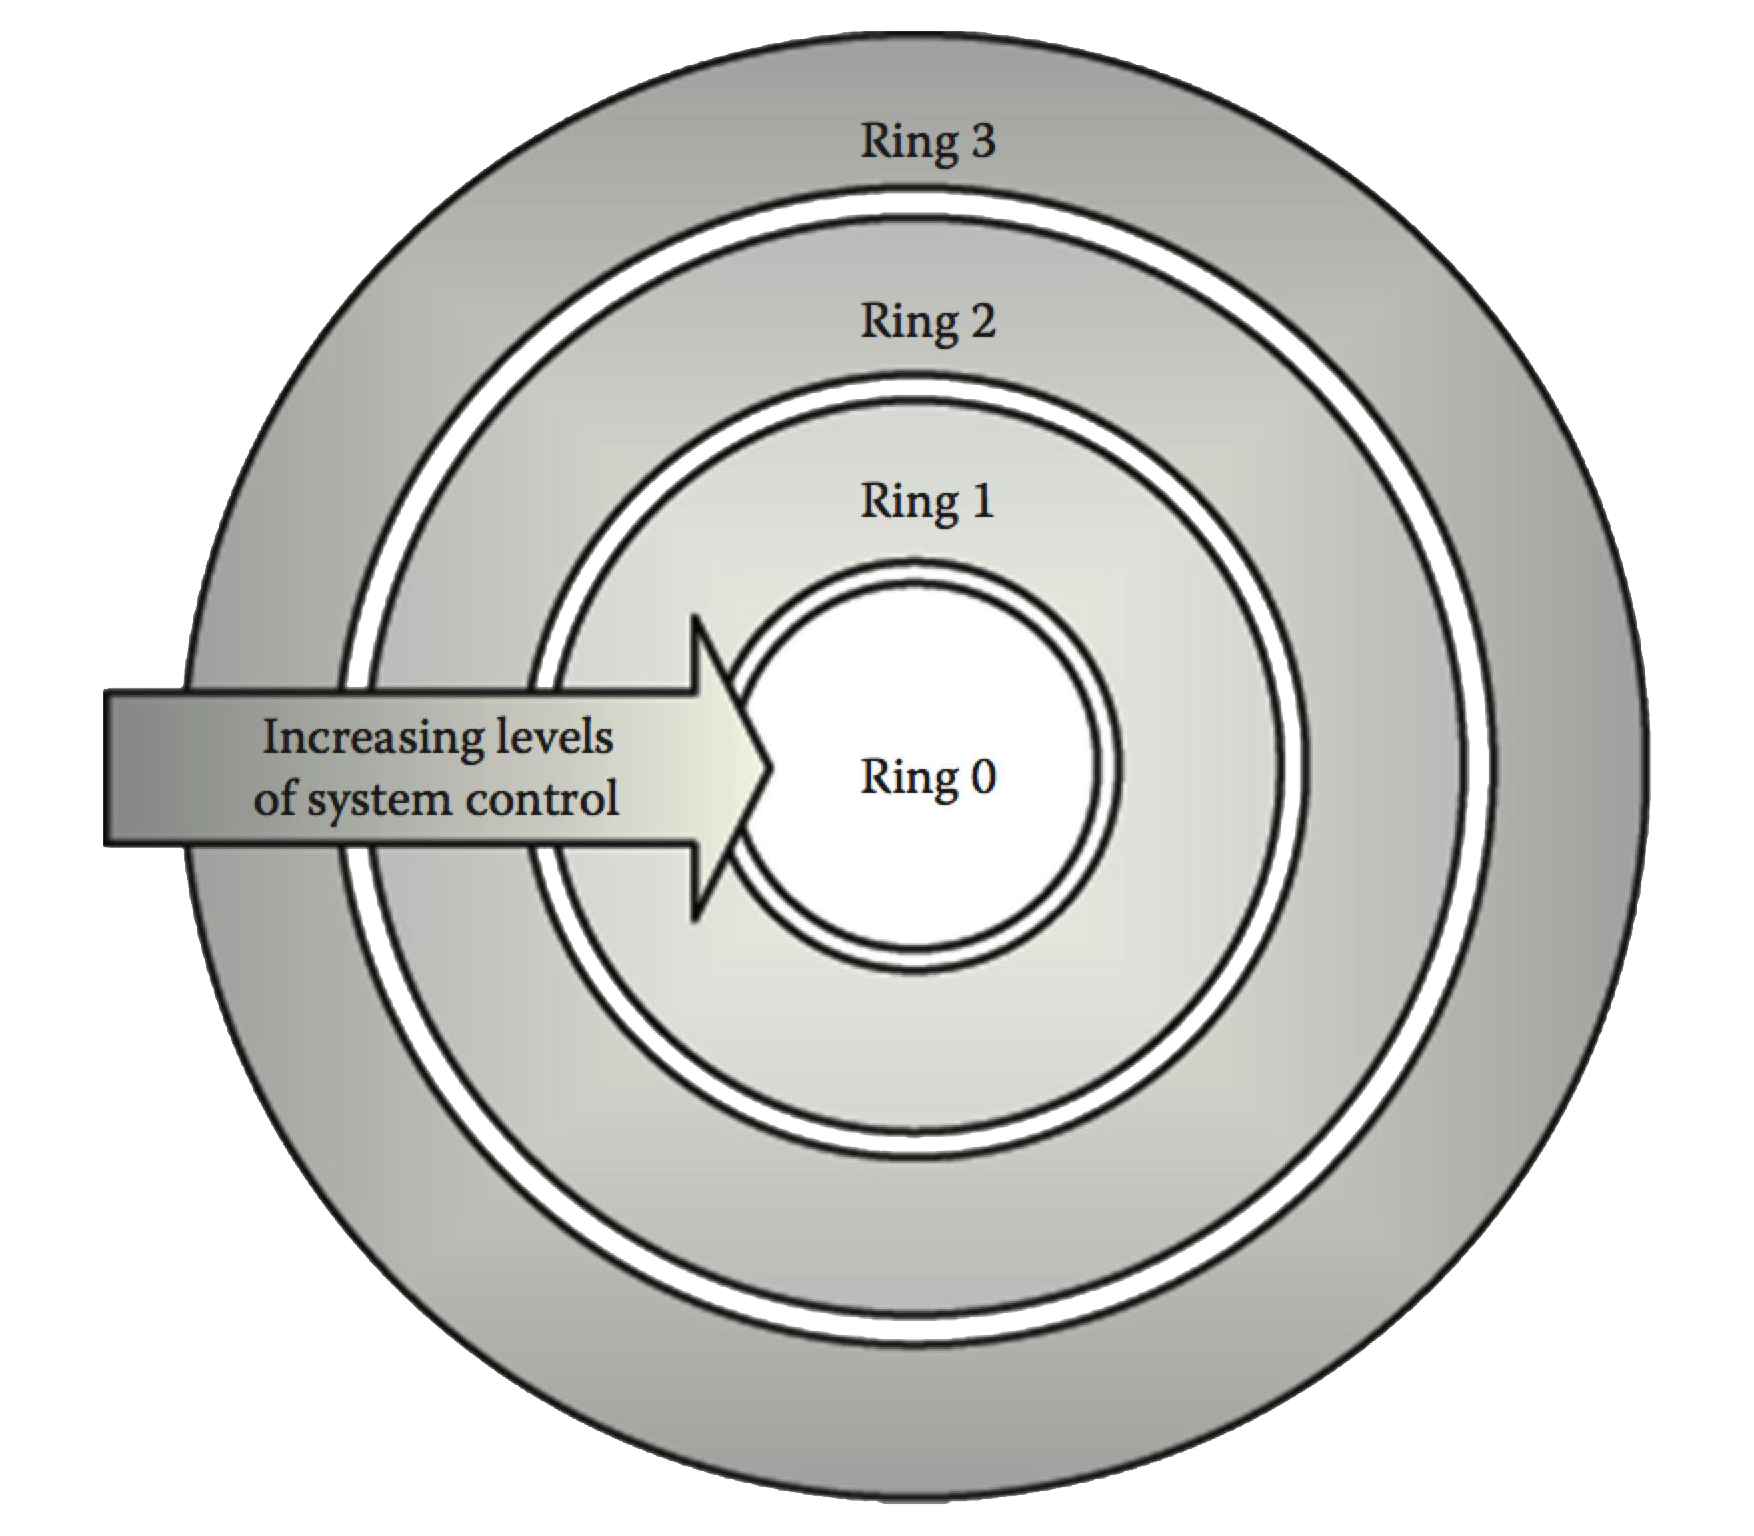
\includegraphics[scale=0.1]{imgs/ring.png}
	\end{figure}
\end{frame}


\begin{frame}
  \frametitle{Building blocks}
  \begin{itemize}[<+- | alert@+>]
  \item Authentication
  \begin{itemize}[<+- | alert@+>]
  \item Verifica dell'identità di una persona o di un servizio che richiede l'accesso ad una risorsa
  \item Autenticazione non solo per l'utente ma anche tra sistemi, processi o componenti hardware
  \end{itemize}
 \item Authorization
 	\begin{itemize}
 		\item Verifica di ciò che la persona o il servizio autenticato può fare all'interno del contesto del sistema
 	\end{itemize}
  \end{itemize}
\end{frame}

\begin{frame}
  \frametitle{Building blocks}
  \begin{itemize}[<+- | alert@+>]
  \item Auditing
  \begin{itemize}
  \item Revisione periodica dell'efficacia dei meccanismi di sicurezza della Smart Grid
  \item Testing delle componenti essenziali per mettere in sicurezza le operazioni
  \end{itemize}
 \item Key management
 	\begin{itemize}
 		\item Gestione dell'emissione delle chiavi per utenti, applicazioni e dispositivi
 		\item Stabilire l'identità dell'utente e garantire l'integrità dei messaggi
 		\item Impiego di Public Key Infrastructure
 	\end{itemize}
  \end{itemize}
\end{frame}

\begin{frame}
  \frametitle{Building blocks}
  \begin{itemize}[<+- | alert@+>]
  \item Message integrity
  \begin{itemize}
  \item Signing
  	\begin{itemize}
  	\item Messaggio inviato da un sistema ad un altro $\rightarrow$ autenticazione $\rightarrow$ autorizzazione $\rightarrow$ scambio di messaggi
  	\end{itemize}
  \item Nonrepudiation
    \begin{itemize}
  	\item Mittente riconosciuto tramite una prova inconfutabile della sua identità
  	\end{itemize}
  \item Encryption
    \begin{itemize}
  	\item Messaggio non può essere letto da una persona/sistema non diretto destinatario
  	\end{itemize}
 	\end{itemize}
  \end{itemize}
\end{frame}

\begin{frame}
  \frametitle{Building blocks}
  \begin{itemize}[<+- | alert@+>]
  \item Network integrity
  \begin{itemize}
  \item Firewall
  \item Rilevamento e prevenzione delle intrusioni
 	\end{itemize}
   \item System integrity
     \begin{itemize}
  \item Protezione da malware
  \item Gestione della configurazione del sistema
  \item Validazione e testing
 	\end{itemize}
  \end{itemize}
\end{frame}

\begin{frame}{Smart Grid Cybersecurity: Sommario}
\begin{itemize}
\item Stuxnet
\item Definire la sicurezza
	\begin{itemize}
	\item Confidentiality
	\item Integrity
	\item Availability
	\item Control
	\item Authenticity
	\item Usability
	\end{itemize}
\item Building blocks
	\begin{itemize}
		\item Layered security model
		\item Authentication
		\item Authorization
		\item Auditing
		\item Key management
		\item Message, Network and System integrity
	\end{itemize}
\alert<1>{\item Threats and impacts}
	\begin{itemize}
		\alert<1>{\item Consumer threats}
		\alert<1>{\item Utility companies threats}
	\end{itemize}
\end{itemize}
\end{frame}

\begin{frame}
  \frametitle{Threats and Impacts: Consumer threats}
  \begin{itemize}[<+- | alert@+>]
  \item Minacce naturali
	\begin{itemize}
	\item Venti, tempeste, tornadi e terremoti
%	\item Eliminare totalmente i danni causati da tali calamità non è possibile
%	\item Di critica importanza la definizione di programmi di aiuto in caso di incidenti
	\end{itemize}
	 \item Minacce da singoli o da organizzazioni
	\begin{itemize}
	\item Ladri e stalker
	\item Hacker
	\item Terrorismo
	\item Governo
	\item Società di servizi, in particolare i lavoratori
	\end{itemize}
  \end{itemize}
\end{frame}

%\begin{frame}
%  \frametitle{Threats and Impacts: Consumer threats}
%  \begin{itemize}[<+- | alert@+>]
%  \item \textit{Minacce da singoli o da organizzazioni}
%	\begin{itemize}
%	\item Ladri e stalker
%	\item Hacker
%	\item Terrorismo
%	\item Governo
%	\item Società di servizi, in particolare i lavoratori
%	\end{itemize}
%  \end{itemize}
%\end{frame}

%%%%meno testo, più parole chiave da qui in giù. Parole tolte usate a voce

\begin{frame}
  \frametitle{Threats and Impacts: Consumer threats - Impatti}
	\textbf{Privacy del consumatore}
		\begin{itemize}
		\item Raccolta di informazioni personali
		\item Attaccante può utilizzarli per scopi malevoli
		\end{itemize}
		\pause
	\textbf{Impatto sull'availability}
			\begin{itemize} 
		\item Obiettivo Smart Grid: disponibilità perenne di corrente
		\item Attacchi possono causare: alterazione di termostati, limitazione di servizi d'emergenza
		\end{itemize}
		\pause
	\textbf{Impatto finanziario}
				\begin{itemize}
		\item Corruzione di dati $\rightarrow$ emissione di bollette inaccurate
		\end{itemize}
\end{frame}

\begin{frame}
  \frametitle{Threats and Impacts: Utility companies threats}
 \textbf{\textit{Confidentiality}}
  \begin{itemize}[<+- | alert@+>]
	  \item Privacy del consumatore
	  \begin{itemize}
	  \item Attacco alla Web application della società 
	  \item Analisi dello storico dei consumi $\rightarrow$ identificare comportamenti utente
	  \end{itemize}
	\item Informazioni proprietarie
		\begin{itemize}
		\item Segreto aziendale $\rightarrow$ target appetibile per hacker
		\end{itemize}
 	\end{itemize}
\end{frame}

\begin{frame}
  \frametitle{Threats and Impacts: Utility companies threats}
  \textbf{\textit{Integrity}}
  \begin{itemize}[<+- | alert@+>]
	  \item Frode
	  \begin{itemize}
	  \item Manomissione dello smart meter per sottostimare i consumi $\rightarrow$ bollette meno costose 
	  \item Modifica dati relativi alla produzione di energia $\rightarrow$ compensi maggiori
	  \end{itemize}
	\item Manipolazione dei dati dei sensori
		\begin{itemize}
		\item Simulare un guasto $\rightarrow$ la società spende tempo e denaro per le riparazioni
		\end{itemize}
 	\end{itemize}
\end{frame}

\begin{frame}
  \frametitle{Threats and Impacts: Utility companies threats}
  \textbf{\textit{Availability}}
  \begin{itemize}[<+- | alert@+>]
	\item Clienti
	  	\begin{itemize}
	  	\item Connessione allo smart meter di un utente $\rightarrow$ cambio password + spegnimento corrente
	  	\end{itemize}
	\item Organizzazioni
			\begin{itemize}
			\item Hacker che vuole danneggiare la società $\rightarrow$ \textit{Denial of Service attack}
			\item Ex dipendente di un'azienda
			\end{itemize}
	\item Manipolazione del mercato
		\begin{itemize}
		\item Team di hacker + esperti di mercati finanziari $\rightarrow$ Ottenere significative quantità di denaro in poco tempo
		\end{itemize}
 	\end{itemize}
\end{frame}


\section{Standard e tecnologie}
\begin{frame}{Standard e tecnologie: Sommario}
	\begin{itemize}
		\item Tecnologie di comunicazione
		\begin{itemize}
			\item IEEE 802
			\begin{itemize}
				\item Ethernet
				\item Wireless
				\item Bluetooth
				\item ZigBee \& 6LoWPAN
				\item WiMAX
			\end{itemize}
			\item Power Line Communication
		\end{itemize}
		\item Standard per lo scambio di informazioni
		\begin{itemize}
			\item Modbus
			\item ISO/IEC 61850
		\end{itemize}
		\item Standard per la sicurezza
		\begin{itemize}
			\item ISO/IEC 62351
		\end{itemize}
	\end{itemize}
\end{frame}

\plain{Tecnologie di comunicazione}
\begin{frame}{IEEE 802}
	\begin{itemize}
		\item Famiglia di standard sviluppati per il supporto alle reti locali
		\item L'architettura è incentrata sui due livelli inferiori del modello ISO/OSI
	\end{itemize}
	\begin{figure}[h] 
		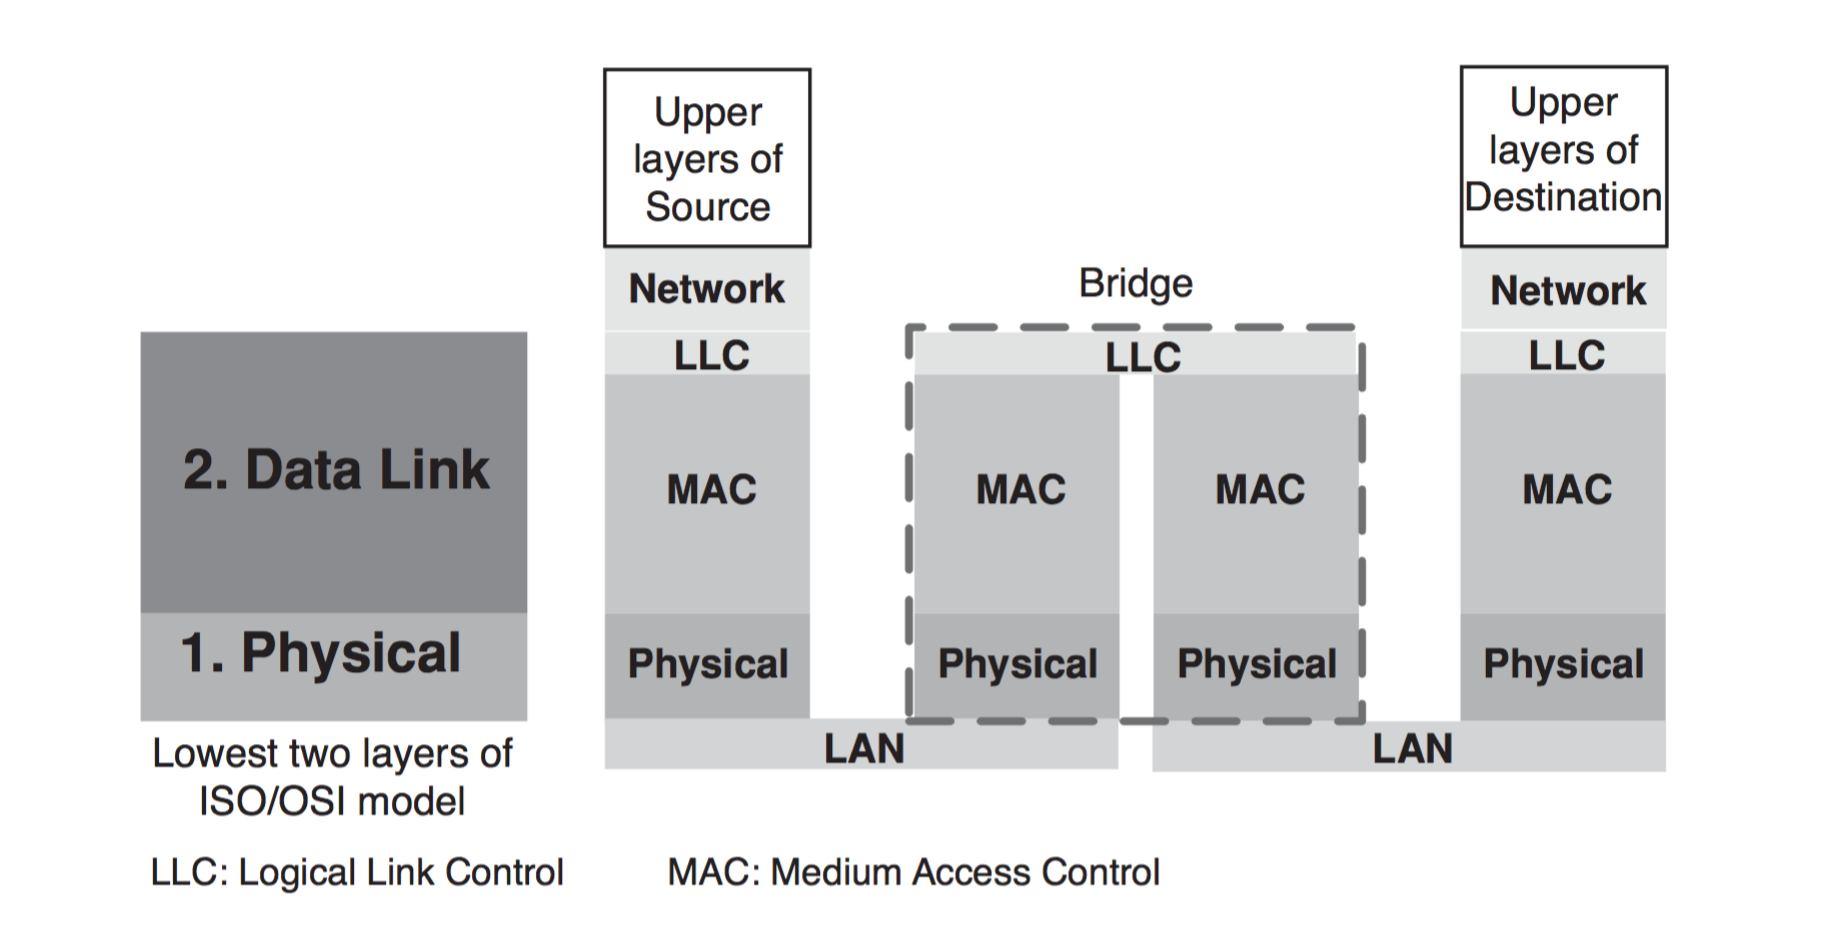
\includegraphics[scale=0.3,cfbox=blue_slides 1pt 0pt]{imgs/arch_ieee802.png}
	\end{figure}
\end{frame}

%Un set di host connessi ad una rete in modo tale che la trasmissione simultanea da due host nel set porta a collisioni, crea un dominio di collisione. Inoltre, le LAN Ethernet trasportano anche frame di broadcast il cui dominio raggiungibile è chiamato dominio di broadcast.
%Le prestazioni della rete, in caso di traffico, sono influenzate dal modo in cui i domini di collisione e di broadcast sono posizionati e pertanto l’idea è quella di isolarli per aumentare le prestazioni della rete
%I Bridge limitano i domini di collisione mentre i Router limitano entrambi i domini
\begin{frame}{IEEE 802[.3]}
	\textbf{Ethernet}
	\begin{block}{}
		Xerox Corporation, Intel Corporation e la Digital Equipment Corporation nel 1978 portarono alla standardizzazione di 802.3 e nel 1980 ci fu la pubblicazione della versione 1.0 dello standard Ethernet
	\end{block}
	\begin{itemize}
		\item Una tra le tecnologie di rete più utilizzate per le LAN cablate
		\item Frame-based
		\item Utilizza un mezzo condiviso (collisioni gestite da \textit{CSMA/CD})
	\end{itemize}
	\begin{figure}[h] 
		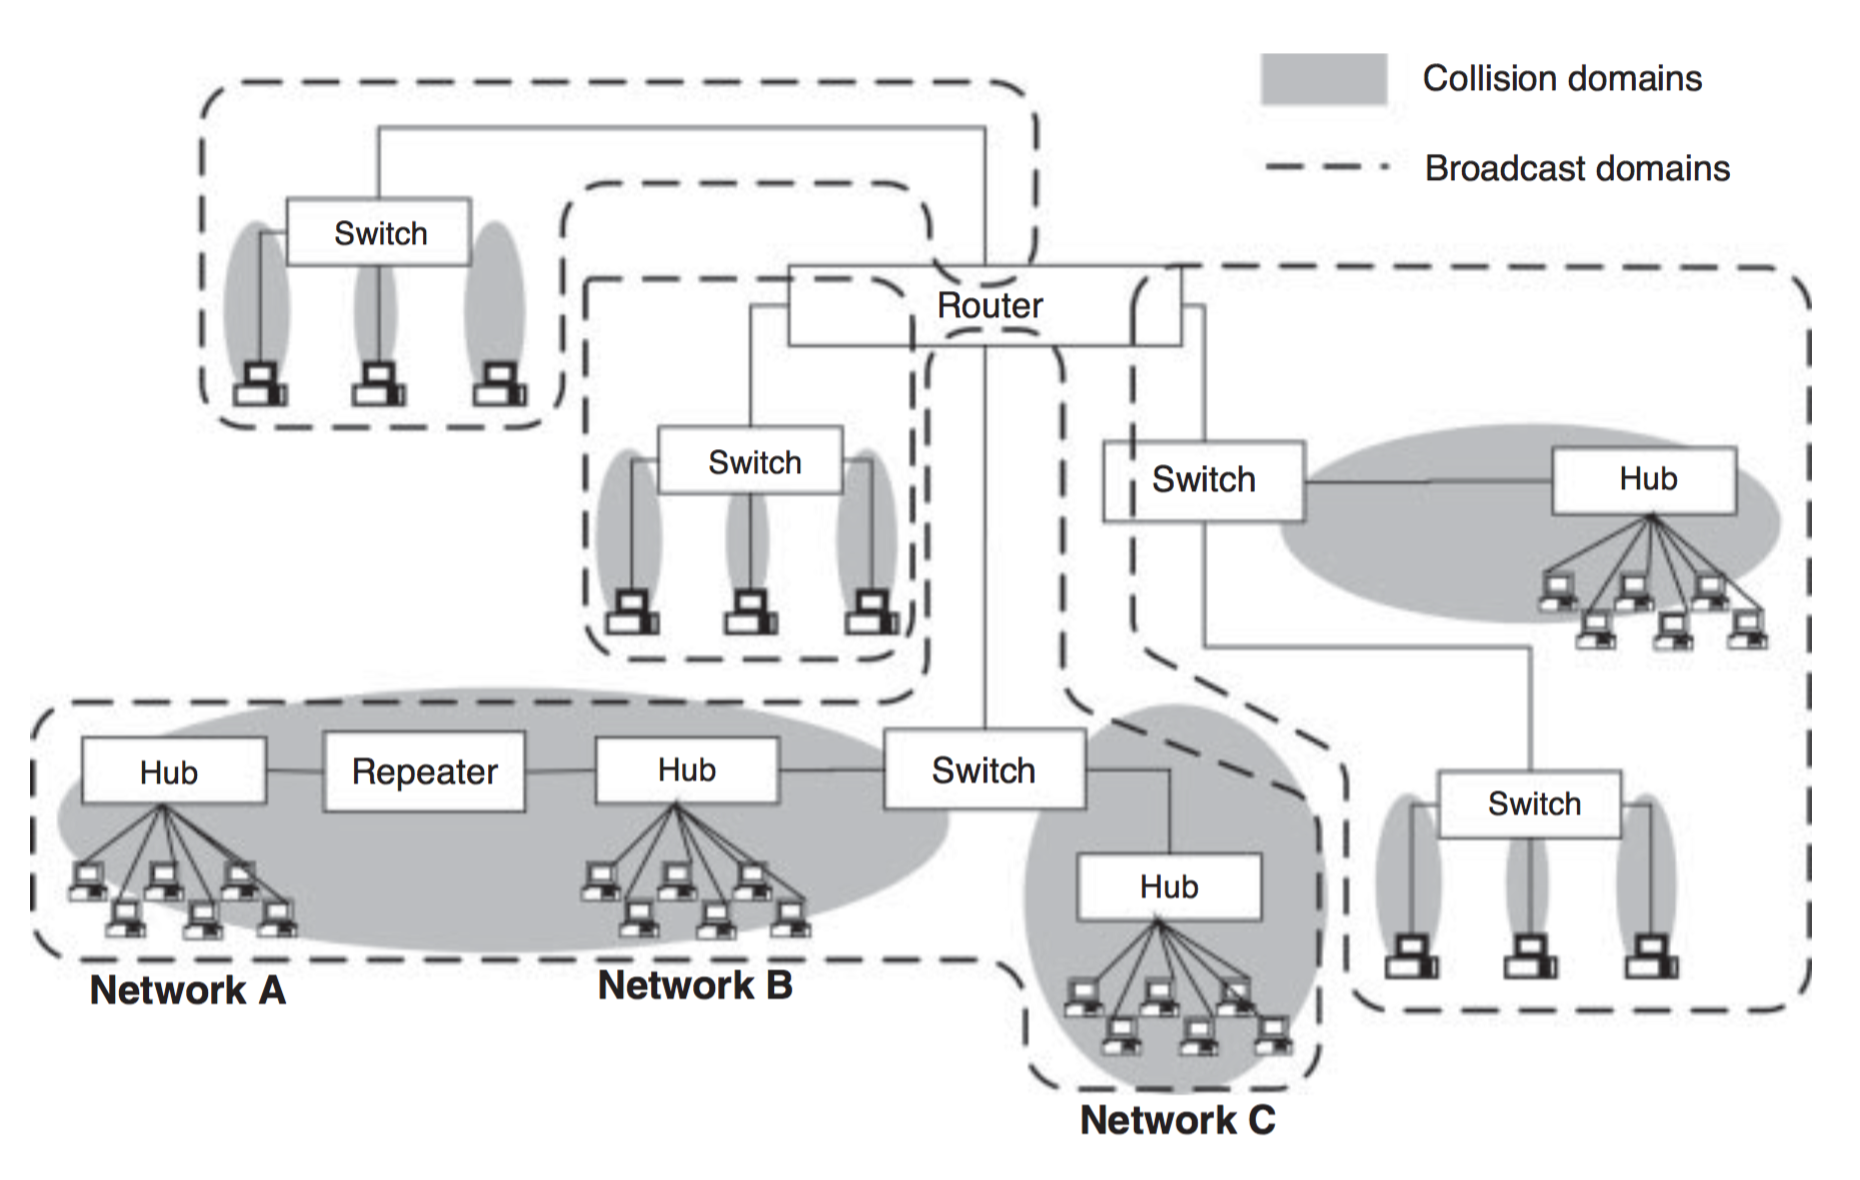
\includegraphics[scale=0.15,cfbox=blue_slides 1pt 0pt]{imgs/lan.png}
	\end{figure}
\end{frame}


\begin{frame}{IEEE 802[.11]}
	\textbf{Wireless}
	\begin{block}{}
	Vic Hayes è stato coinvolto nella progettazione degli standard 802.11a e 802.11b  all'interno di IEEE nel settembre del 1999
	\end{block}
	\pause
	\begin{itemize}[<+- | alert@+>]
		\item Definisce un insieme di standard per le Wireless LAN
		\item Utilizza un mezzo condiviso (collisioni gestite da \textit{CSMA/CA})
		\item Componenti:
			\begin{itemize}
				\item Station
				%Qualsiasi dispositivo che comunica tramite una rete WLAN, ad esempio, un computer portatile, o cellulari che supportano WiFi
				\item Access Point (\textbf{BSS}) 
				%Consente ad una stazione di comunicare con un altra facendo da tramite
				%Gli AP rendono il sistema scalabile e consentono la connessione cablata con altre reti
				%In presenza di AP l’insieme delle station è chiamato Infrastructure BSS
				\item Distribution System (\textbf{ESS})
				%Interconnette Infrastructure BSS attraverso gli AP
				%Facilita la comunicazione tra gli AP, l’inoltro del traffico da un BSS ad un altro ed il movimento di mobile station tra BSS
				%Un insieme di Infrastructure BSS è chiamato Extended Service Set (ESS)
			\end{itemize}
	\end{itemize}
\end{frame}
\begin{frame}{IEEE 802[.11]}
	\textbf{Wireless}
	\newline
	Basic Service Set (BSS)
		\begin{figure}[h] 
			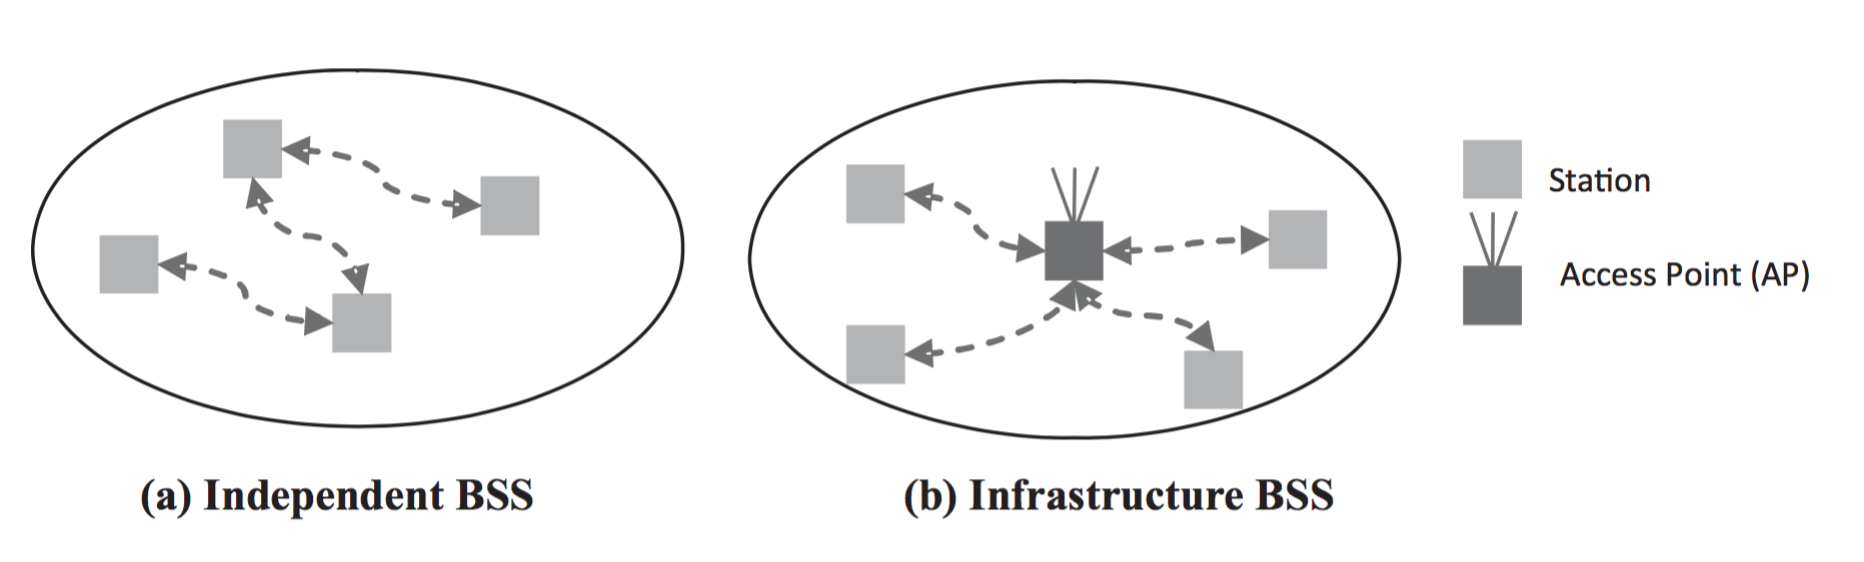
\includegraphics[scale=0.3,cfbox=blue_slides 1pt 0pt]{imgs/bss.png}
			%\caption{Architettura BSS}
		\end{figure}
	\end{frame}
	\begin{frame}{IEEE 802[.11]}
	\textbf{Wireless}
	\newline
	Distribution System
		\begin{figure}[h] 
			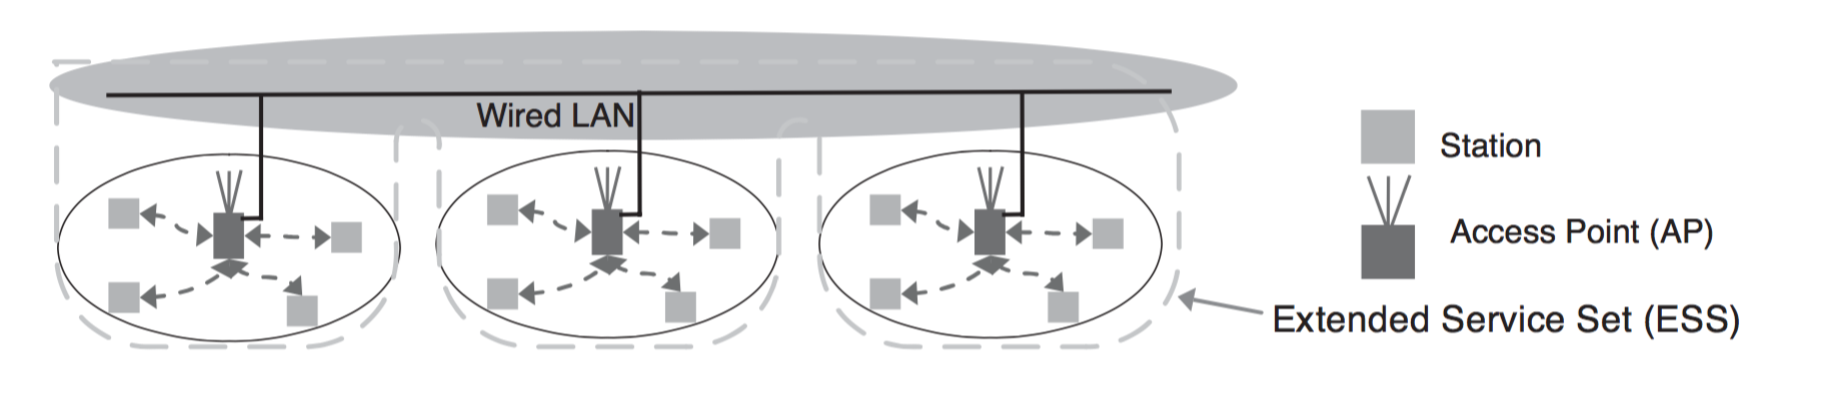
\includegraphics[scale=0.3,cfbox=blue_slides 1pt 0pt]{imgs/ds.png} %border color
		\end{figure}
\end{frame}
	
\begin{frame}{IEEE 802[.15.1]}
	\textbf{Bluetooth}
	\begin{block}{}
		Inventato da Ericsson nel 1994, originariamente concepito come un' alternativa senza fili ai cavi RS-232
	\end{block}
	\pause
	\begin{itemize}[<+- | alert@+>]
		\item Tecnologia wireless progettata per collegare dispositivi mobili o fissi
			\begin{itemize}[<+- | alert@+>]
				\item Bassi consumi
				\item Corto raggio d'azione
				\item Basso costo di produzione per dispositivi compatibili
			\end{itemize}
			\item Presenta due architetture di Rete
			\begin{itemize}[<+- | alert@+>]
				\item Piconet
				\begin{itemize}
					\item Un dispositivo \textit{Master}
					\item Fino a sette dispositivi \textit{Slave}
		%Altri dispositivi possono sincronizzarsi col Master ma non possono partecipare alla comunicazione, tali dispositivi sono in un parked state
		%Un device in parked state può passare in active state se il numero di Slave della Piconet è inferiore a sette
				\end{itemize}
				\item Scatternet
				\begin{itemize}[<+- | alert@+>]
					\item Un insieme di \textbf{Piconet}
				\end{itemize}
			\end{itemize}
	\end{itemize}		
\end{frame}

%	Un dispositivo si può trovare in due stati:
%Connessione: Active mode, Hold mode, Sniff mode, Park mode
%Standby: Ascolta il canale ogni 1,28 secondi per eventuali messaggi dal Master

\begin{frame}{IEEE 802[.15.1]}
\textbf{Bluetooth}
	\begin{figure}[h] 
		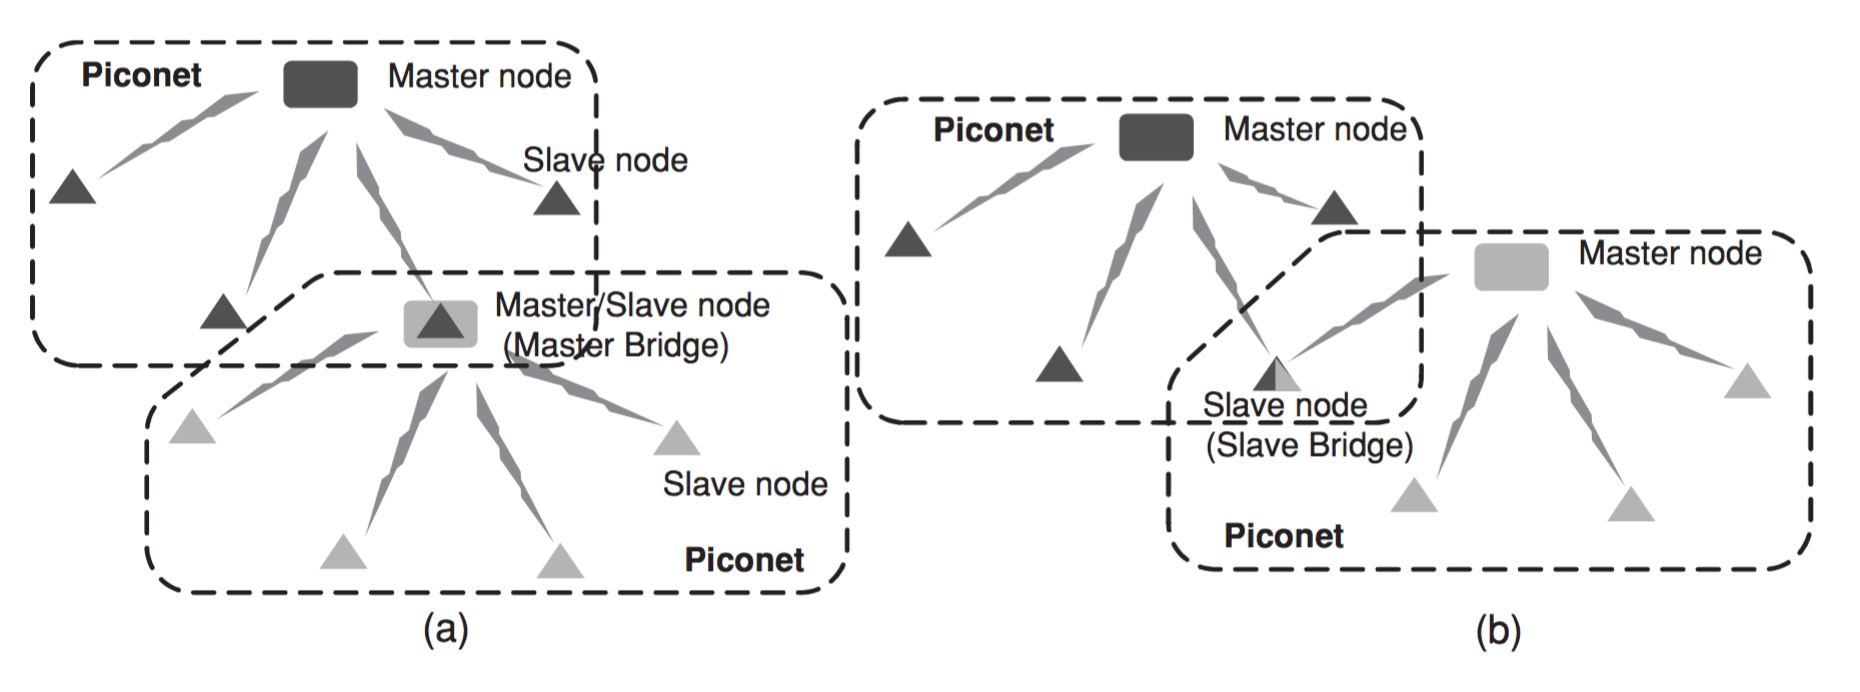
\includegraphics[scale=0.3,cfbox=blue_slides 1pt 0pt]{imgs/bt.png}
		%Le Piconet possono essere interconnesse attraverso un Bridge che può essere Slave per una Piconet e Master per un’altra oppure Slave per due Piconet
	\end{figure}
\end{frame}

\begin{frame}{IEEE 802[.15.4]}
\textbf{ZigBee \& 6LoWPAN}
	\newline
	Sono due tecnologie per Wireless Private Area Network (WPAN)
	\begin{itemize}[<+- | alert@+>]
		\item Basso consumo
		\item Alta flessibilità
		\item Bassi costi
	\end{itemize}
\end{frame}

\begin{frame}{IEEE 802[.15.4]}
\textbf{ZigBee}
\begin{block}{}
La prima specifica fu ratificata il 14 dicembre 2004. La ZigBee Alliance annuncia la disponibilità della specifica 1.0 il 13 giugno 2005%alla quale successivamente vennero rilasciate due versioni nel 2007.
\end{block}
%Considerata come una buona opzione per il metering e per la gestione dell’energia ideale in implementazioni Smart Grid data la semplicità, mobilità, robustezza e i bassi costi di sviluppo.
%Problematiche: basse capacità elaborative, piccola dimensione della memoria e interferenze.
\begin{itemize}
	\item \textit{Application Support} e \textit{Network Layer} sono definiti dalla ZigBee Alliance
	\item Un device può essere di due tipi
	\begin{itemize}
		\item Full Function Device (FFD)
			\begin{itemize}
				\item Coordinatore, Router, Device
				\item Può interagire sia con un FFD che con un RFD
			\end{itemize}
		\item Reduced Function Device (RFD)
			\begin{itemize}
				\item Device
				\item Può interagire solo con un FFD
			\end{itemize}
	\end{itemize}
\end{itemize}
	\begin{figure}[h] 
		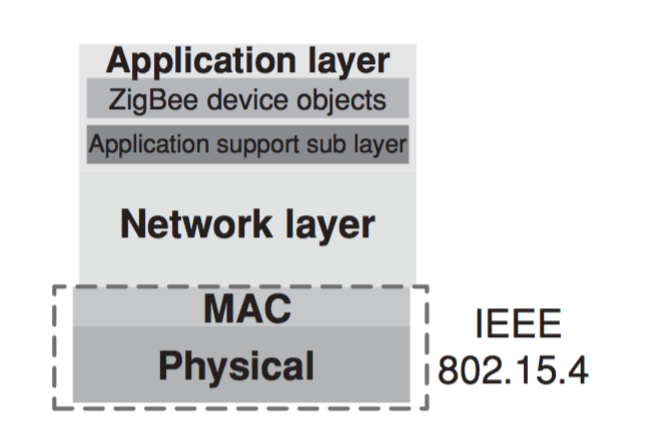
\includegraphics[scale=0.2,cfbox=blue_slides 1pt 0pt]{imgs/zbprot.png}
		%\caption{Architettura protocollare di ZigBee}
	\end{figure}
\end{frame}


%RFD vuole inviare un pacchetto al di fuori del dominio 6LoWPAN.
%RFD -> FFD(router) nella stessa WPAN -> gateway 6LoWPAN che inoltrerà al dispositivo destinatario tramite IP
\begin{frame}{IEEE 802[.15.4]}
	\textbf{6LoWPAN}
	\begin{block}{}
		Il gruppo di lavoro IETF 6LoWPAN è stato approvato nel marzo del 2005. Nel 2009 la ZigBee Alliance ha annunciato l'integrazione di ZigBee con 6LoWPAN
	\end{block}
	\begin{itemize}
		\item Consente l'invio e la ricezione di pacchetti \textit{IPv6}
		\item E' stato inserito un Adaptation Layer per il collegamento tra lo strato \textit{MAC} e il \textit{Network Layer IPv6}
	\end{itemize}
	\begin{figure}[h]
		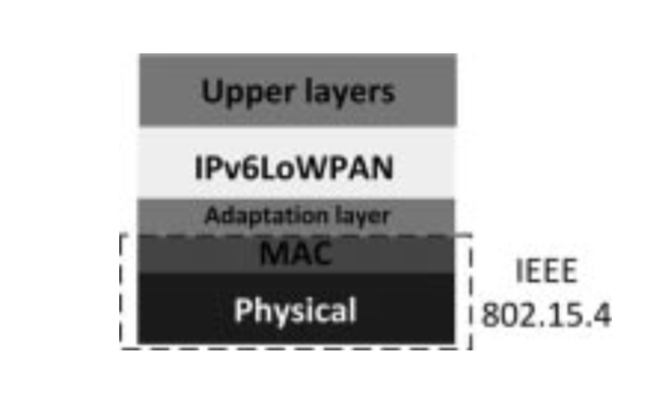
\includegraphics[scale=0.3,cfbox=blue_slides 1pt 0pt]{imgs/6pan.png}
	\end{figure}
\end{frame}

\begin{frame}{IEEE 802[.16]}
	\textbf{WiMAX}
	\begin{block}{}
		Prima pubblicazione effettuata dal WiMAX Forum l'8 aprile del 2002 con lo standard IEEE 802.16-2001
	\end{block}
	\pause
	\begin{itemize}[<+- | alert@+>]
		\item Tecnologia wireless adatta a trasmissione sia di tipo urbano che rurale
		\item Implementa diverse tecniche di crittografia, sicurezza ed autenticazione
		\item Tecnica di Orthogonal Frequency Division Multiple Access (OFDMA)
		\item Soddisfa varie specifiche imposte da una tipica Smart Grid
		%Tra cui massima accessibilità ed interoperabilità, tempi di latenza inferiori ai 50 ms e larghezza di banda di 5 MHz.
		%La copertura si estende fino ai 50 km
		%Supporta i dispositivi mobili
	\end{itemize}
\end{frame}

\begin{frame}{IEEE 802[.16]}
	\textbf{WiMAX}
	\begin{figure}[h]
		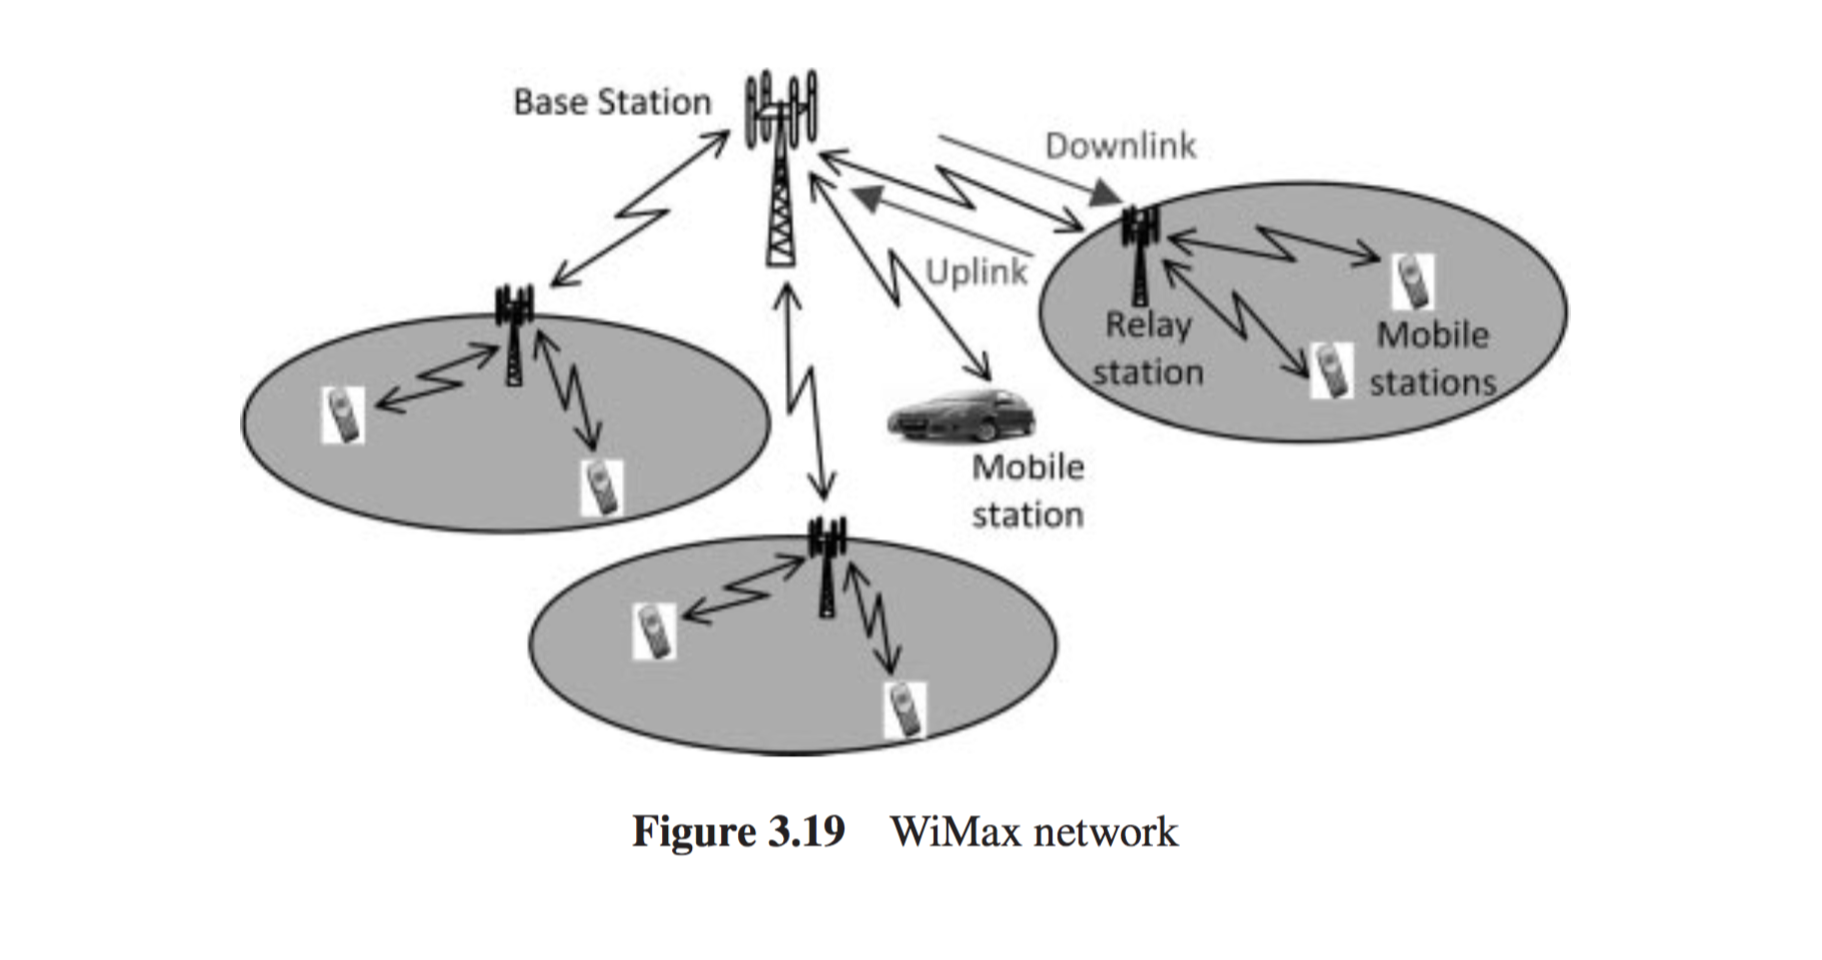
\includegraphics[scale=0.3,cfbox=blue_slides 1pt 0pt]{imgs/wim.png}
	\end{figure}
\end{frame}

%IEEE P1901 e HomePlug
%L’ENEL, nota azienda multinazionale produttrice e distributrice di energia elettrica, ha scelto la tecnologia PLC per trasferire i dati degli smart meter al data concentrator più vicino e la tecnologia GSM per inviare i dati al data center.
%Sono utilizzate tre tecnologie di comunicazione che prendono il nome di narrowband transmission, spread-spectrum transmission e DSP-processed narrowband transmission
\begin{frame}{Power line}
	\textbf{Power Line Communication}
	\begin{block}{}
	I primi standard sono stati progettati nel 2001 dalla Homeplug Powerline Alliance
	%l'Homeplug 1.0 e l'HomePlug 1.0 Turbo, per trasferire dati a una velocità teorica rispettivamente di 15 e 85 Mbit/secondo
	%Dopo alcuni anni di competizione serrata sugli standard, i due standard al di sopra i 200 Mbs sono confluiti in un unico standard internazionale IEEE P1901 Powerline AV, cui rispondono ormai tutti i prodotti in commercio come HPAV Powerline HomePlug AV
	\end{block}
	\pause
	\begin{itemize}[<+- | alert@+>]
		\item Tecnologia di rete proposta per la trasmissione in ambiente Smart Grid
		\item Trasporto informazioni su conduttori e linee elettriche %risparmio dal punto di vista di creazione dell'infrastruttura
		\item Servizi di comunicazione per AMI e HAN
	\end{itemize}
	\pause
	\begin{block}{}
		\textit{In una tipica rete \textbf{\color{blue_slides}PLC}, gli smart meter sono collegati al data concentrator attraverso power line e i dati vengono trasferiti al data center tramite tecnologie di rete cellulare}
	\end{block}
	\pause
	\begin{block}{Problema}
		Presenza di disturbi che possono corrompere le informazioni, non garantendo più la continuità del servizio
	\end{block}
\end{frame}

\plain{Standard per lo scambio di informazioni}

%DNP3
%Insieme di protocolli di comunicazione utilizzato tra i componenti nei sistemi di automazione
%Fondamentale nei sistemi SCADA, utilizzato dalle Master Station per comunicare con le RTU e gli IED
%	Lo User Layer DNP prende input analogici/binari e da in output segnali analogici e binari.
%Un master dnp3 invia richieste e le stazioni Slave rispondono, ma uno Slave può anche trasmettere messaggi senza aver ricevuto richiesta.
%Il Physical Layer utilizza noti protocolli di comunicazione seriali come EIA 232 o EIA 485.

\begin{frame}{Standard per lo scambio di informazioni}
	\textbf{Modbus}
	\begin{block}{}
	Protocollo creato nel 1979 da Modicon (azienda ora parte del gruppo \textbf{\color{blue_slides}Schneider Electric})
	\end{block}
	\pause
	\begin{itemize}[<+- | alert@+>]
		\item Protocollo di messaggistica (\textit{Application Layer})%risiede nell’Application Layer e consente la comunicazione tra i dispositivi collegati su diversi bus e reti
		\item Dispositivi collegati su diversi bus e reti%protocollo utilizzato per mettere in comunicazione i controllori logici programmabili
		\item Ethernet su fibra ottica con trasmissione seriale asincrona%EIA 232, EIA 422, EIA 485
		\item Automazione delle substation%Modbus su EIA 485
		\item Comunicazione
			\begin{itemize}[<+- | alert@+>]
			\item Master $\xrightarrow{query}$ Slave/broadcast
			\item Slave (monitoring delle \textit{query})
			\item Slave $\xrightarrow{trigger}$ azione
			\end{itemize}
	\end{itemize}
\end{frame}


%Generalmente, questi protocolli girano su reti TCP/IP o LAN con switch Ethernet molto performanti per rispondere ai requisiti stringenti dei dispositivi, che necessitano di tempi di risposta inferiori a 4-5 millisecondi.
\begin{frame}{Standard per lo scambio di informazioni}
	\textbf{ISO/IEC 61850}
	\begin{block}{}
		Un gruppo IEC di 60 membri si è diviso in 3 gruppi di lavoro per la creazione di ISO/IEC 61850 nell'1995
	\end{block}
	\pause
	\begin{itemize}[<+- | alert@+>]
		\item Progettazione dei sistemi di automazione per le substation
		\item Sovrastruttura che coordina e gestisce protocolli e tecnologie esistenti
		\item Garantisce interoperabilità
	\end{itemize}
\end{frame}

\begin{frame}{Standard per lo scambio di informazioni}
	\textbf{ISO/IEC 61850}
	\begin{block}{Vantaggi}
	\begin{itemize}[<+- | alert@+>]
		\item Coordina la complessità di unità indipendenti
		\item Si integra con sistemi preinstallati in rete
		\item Scalabile e facilita integrazione
		\item Si basa su standard esistenti
		\item Supporta i \textit{self descriptive device}%eliminando problemi di configurazione manuale
		\item Si basa su \textit{data object}%e standardizzazione degli elementi tipici di una rete elettrica
		\item Estensibile e flessibile
		\item Si adatta rapidamente alla configurazione del sistema
	\end{itemize}
	\end{block}
\end{frame}

%ISO/IEC 61850 suddivide ogni sottostazione in tre livelli[25] chiamati Station Level, Bay Level e Process Level

%Un device model considera inizialmente un physical device. Tale modello consente ad un singolo dispositivo fisico di agire da gateway di informazioni per più dispositivi. Successivamente vengono specificati i logical device all’interno di tale dispositivo. Ogni logical device contiene uno o più logical node, logicamente correlati ad una funzione della stazione. I logical node sono definiti da gruppi di data object e relativi servizi, ognuno modellato secondo gli schemi definiti dalle Common Data Classes (CDC).

%I logical node sono identificati con nomi definiti dallo standard in cui la prima lettera indica l’attinenza (e.g. A controllo automatico, M misura, X switchgear, etc)

%Utilizzando tale formato si è in grado di indicare le informazioni relative allo status o alla posizione di un dispositivo
\begin{frame}{Standard per lo scambio di informazioni}
\textbf{ISO/IEC 61850}
	\newline\textbf{Device Model}
	\begin{figure}[h] 
		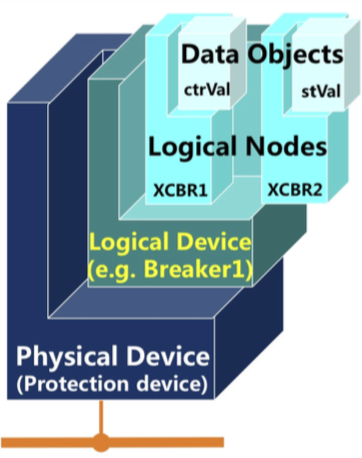
\includegraphics[scale=0.35,cfbox=blue_slides 1pt 0pt]{imgs/iec61850ln.png}
	\end{figure}
\end{frame}

\begin{frame}{Standard per lo scambio di informazioni}
\textbf{ISO/IEC 61850}
	\begin{itemize}[<+- | alert@+>]
		\item Oggetti e servizi astratti di comunicazione %permettono di scrivere un'applicazione indipendentemente dai protocolli tradizionali.
		\item Abstract Communication Service Interface (ACSI)
			\begin{itemize}[<+- | alert@+>]
				\item Oggetti e servizi implementati attraverso il protocollo Manufacturing Message Specification (MMS) 
				%Che definisce i messaggi di comunicazione tra i centri di controllo o tra stazioni e centri
			\end{itemize}
		\item Linguaggio comune di configurazione per astrazione e standardizzazione
		\begin{itemize}[<+- | alert@+>]
			\item Substation Configuration Language (SCL)%basato su XML
			\begin{itemize}[<+- | alert@+>]
			\item[+] Interoperabilità tra IED
			\item[+] Configurazione automatica
			\item[+] Riduzione della presenza di errori
			\end{itemize}
			\item Ogni IED presenta un file SCL che ne definisce la configurazione
		\end{itemize}
	\end{itemize}		
\end{frame}

\begin{frame}{Standard per lo scambio di informazioni}
\textbf{ISO/IEC 61850}
\newline
Lo standard si serve dei seguenti strumenti per la gestione delle informazioni
\begin{itemize}[<+- | alert@+>]
	\item Generic Substation Event (GSE)
	%Protocollo che fornisce uno strumento veloce ed affidabile per la segnalazione di eventi all’interno della sottostazione. Le caratteristiche principali sono il servizio multicast/broadcast con modello di comunicazione publish/subscribe. I messaggi sono trasmessi in formato binario. GSE prevede due modelli di servizio che prendono il nome di GOOSE e GSSE
	\begin{itemize}[<+- | alert@+>]
		\item Generic Object Oriented Substation Event (GOOSE)
		%Utilizza Virtual LAN, stabilendo più network virtuali sulla stessa rete fisica e determinando livelli di priorità per i messaggi, consentendone anche la ritrasmissione
		\item Generic Substation State Event (GSSE)
		%Utilizzato per lo scambio di informazioni sui soli cambiamenti di stato. In questo caso i messaggi sono costituiti da una serie di bit che rap- presentano liste di stati. GSSE necessita un tempo di trasmissione maggiore se confrontato con GOOSE
	\end{itemize}
	\item Sampled Measured Values (SMV)
	%Protocollo per lo scambio di dati e la trasmissione di misure prodotte dai trasduttori delle sottostazioni: permette lo scambio di segnali tra gli IED
	\item Time Synchronization
	%Servizio di sincronizzazione dei clock fondamentale per applicazioni real-time. Utilizza un subset di Network Time Protocol (NTP) con riferimento allo Universal Coordinated Time (UTC). NTP è il protocollo tipicamente utilizzato per sincronizzare i clock di computer collegati ad Internet e in LAN.
	\item Report e Logging
	%REPORT: Strumento che permette di memorizzare i cambiamenti dei dati e degli attributi relativi ai nodi logici. Genera dataset contenenti attributi di interesse e richiede ai nodi logici l’invio delle informazioni riguardanti le variazioni nel sistema
	%LOG: Registrazione degli eventi relativi ad un dispositivo. I log sono registrati in un server e, a differenza dei Report, i dispositivi logici creano al loro interno un database di eventi senza inviarne notifica
\end{itemize}
\end{frame}

\plain{Standard per la sicurezza}

%Di recente invenzione e fondamentali data la grande mole di informazioni sensibili memorizzate sui computer collegati in rete
%Molte attività si sono automatizzate introducendo maggiore bisogno di affidabilità e sicurezza

%Limiti di ISO/IEC 61850: costi elevati per l’installazione dei server e dei dispositivi atti alla gestione dei dati ma anche complessità dal punto di vista dell’architettura
%ISO/IEC 61850 è affiancato da ISO/IEC 62351 che garantisce la sicurezza e specifica i requisiti tecnici che devono essere rispettati dai fornitori

\begin{frame}{Standard per la sicurezza}
	\begin{block}{I problemi relativi alla sicurezza}
	\begin{itemize}
		\item[-] Accessi non autorizzati a informazioni recuperate dagli smart meter
		\item[-] Spegnimento di dispositivi
		\item[-] Attacco alla Smart Grid per causare un'interruzione al regolare passaggio di corrente
	\end{itemize}
	\end{block}		
	\pause
	\begin{block}{I problemi relativi alla privacy}
	\begin{itemize}
		\item[-] Alta frequenza di letture per misurare il consumo energetico
		\item[+] Si cerca di aggregare le informazioni per mascherare i singoli consumi dei meter
	\end{itemize}
	\end{block}		
\end{frame}

\begin{frame}{Standard per la sicurezza}
\textbf{ISO/IEC 62351}
\begin{block}{}
Standard sviluppato nel 1999 dal WG15 facente parte della TC57 dell'organo internazionale IEC
\end{block}
\pause
\begin{block}{Obiettivi di sicurezza}
\begin{itemize}
	\item Autenticazione nel processo di trasferimento di dati tramite firma digitale
	\item Garanzia di accessi esclusivamente dopo autenticazione
	\item Prevenzione dell'\textbf{\color{blue_slides}eavesdropping}%ossia intercettazioni della comunicazione non autorizzate
	\item Prevenzione da attacchi di \textbf{\color{blue_slides}playback} e attacchi di \textbf{\color{blue_slides}spoofing}
	%PLAYBACK (REPLAY ATTACK): Impossessarsi di una credenziale di autenticazione comunicata da un host ad un altro, e riproporla successivamente simulando l'identità dell'emittente	
	%SPOOFING: ovvero sostituirsi ad una controparte della comunicazione
	\item Rilevamento delle intrusioni
\end{itemize}
\end{block}
\end{frame}

\begin{frame}{Standard per la sicurezza}
	\textbf{ISO/IEC 62351}
	\newline
	E'suddiviso in 8 parti:
	\begin{enumerate}[<+- | alert@+>]
		\item Spiegazioni di alcuni scenari
		\item Definizioni di termini
		\item Definizioni di servizi di sicurezza in comunicazione TCP/IP based
		%Definisce come possono essere forniti servizi di sicurezza in una comunicazione TCP/IP based e specifica suite di cifratura
		\item Aumento dei messaggi di sicurezza trasmessi su MMS
		%Definisce procedure, i miglioramenti del protocollo, e gli algoritmi atti a promuovere l’aumento dei messaggi di sicurezza trasmessi su MMS
		%Tali procedure sono relative a Transport e Application Layer, basate su TLS, usate in modo da proteggere le informazioni trasmesse
		\item Comunicazione seriale
		%in cui si vanno a definire ulteriori misure di sicurezza per proteggere l’integrità delle connessioni seriali applicando chiavi hash
		\item ISO/IEC 61850 %profili iso/iec 61850 per la comunicazione non basati su TCP/IP
		\item Network Management%implementa o estende sistemi di intrusion detection
		\item Role-Based access control
		%Approccio a sistemi ad accesso ristretto per utenti autorizzati.
		%Tre regole fondamentali sono definite per il modello RBAC: Assegnazione dei ruoli, Autorizzazione dei ruoli, Autorizzazione alla transazione
	\end{enumerate}
\end{frame}

\section{Principali vulnerabilità delle Smart Grid: \newline attacchi e contromisure}
% OSGP
% Attacking smart meters and smart devices
% False data injection
% Disconnect attack
% Jamming


\begin{frame}{Principali vulnerabilità delle Smart Grid: attacchi e contromisure}
	\begin{itemize}[<+- | alert@+>]
		\item Digitalizzazione delle infrastrutture critiche
		\begin{itemize}
			\item Aggiunta capacità computazione e comunicazione
		\end{itemize}
		\item Dispositivi non critici e disconnessi
		\begin{itemize}
			\item Connessi $\rightarrow$ Dati \textsc{process-critical}
		\end{itemize}
		\item Anello debole della catena
		\begin{itemize}
			\item Smart Meter
		\end{itemize}
		\item Nuova sfida per i produttori
	\end{itemize}
\end{frame}

\begin{frame}{Principali vulnerabilità delle Smart Grid: sommario}
	\begin{itemize}
		\item Security Testing
		\item Open Smart Grid Protocol
		\item False Data Injection
		\item Disconnect Attack
		\item Jamming
	\end{itemize}
\end{frame}

\begin{frame}{Principali vulnerabilità delle Smart Grid: sommario}
	\begin{itemize}
		\alert<1>{\item Security Testing}
		\item Open Smart Grid Protocol
		\item False Data Injection
		\item Disconnect Attack
		\item Jamming
	\end{itemize}
\end{frame}

\begin{frame}{Principali vulnerabilità delle Smart Grid: dispositivi smart}
	\begin{block}{Smart Devices}
		\begin{itemize}
			\item Dispositivi capaci di computare e comunicare
			\item Godono di tutte le feature di un tipico dispositivo connesso alla rete
			\item Possono essere soggetti ad attacchi
		\end{itemize}
	\end{block}
\end{frame}

\begin{frame}{Principali vulnerabilità delle Smart Grid: Security Testing}
	\textbf{Institute for Security and Open Methodologies (ISECOM)}
	\begin{block}{Open Source Security Testing Methodology Manual (OSSTMM)}
		\begin{itemize}
			\item Information Security
			\item Process Security
			\item \textbf{Internet Technology Security}
			\item Communications Security
			\item Wireless Security
			\item Physical Security
		\end{itemize}
	\end{block}
\end{frame}


\begin{frame}{Principali vulnerabilità delle Smart Grid: Security Testing}
\begin{block}{Internet Technology Security}
	\begin{itemize}[<+- | alert@+>]
		\item Penetration Testing
		\begin{itemize}
			\item Kali Linux
		\end{itemize}
		\item Network Surveying
		\begin{itemize}
			\item Wireshark
		\end{itemize}
		\item Port Scanning, Services/System Identification, DoS Testing
		\begin{itemize}
			\item Nmap
		\end{itemize}
%		\item  Identification
%		\item System Identification
%		\begin{itemize}
%			\item Vulnerability Research and Verification
%		\end{itemize}
%		\item Denial of Service Testing
		\item Internet Application Testing
		\begin{itemize}
			\item Nessus
		\end{itemize}
		\item Exploit Testing
		\begin{itemize}
			\item Metasploit
		\end{itemize}
	\end{itemize}
\end{block}
\end{frame}

\begin{frame}{Principali vulnerabilità delle Smart Grid: sommario}
	\begin{itemize}
		\item Security Testing
		\alert<1>{\item Open Smart Grid Protocol}
		\item False Data Injection
		\item Disconnect Attack
		\item Jamming
	\end{itemize}
\end{frame}

\begin{frame}{Principali vulnerabilità delle Smart Grid: comunicazione tra data aggregator e smart meter}
	\begin{figure}[h] 
		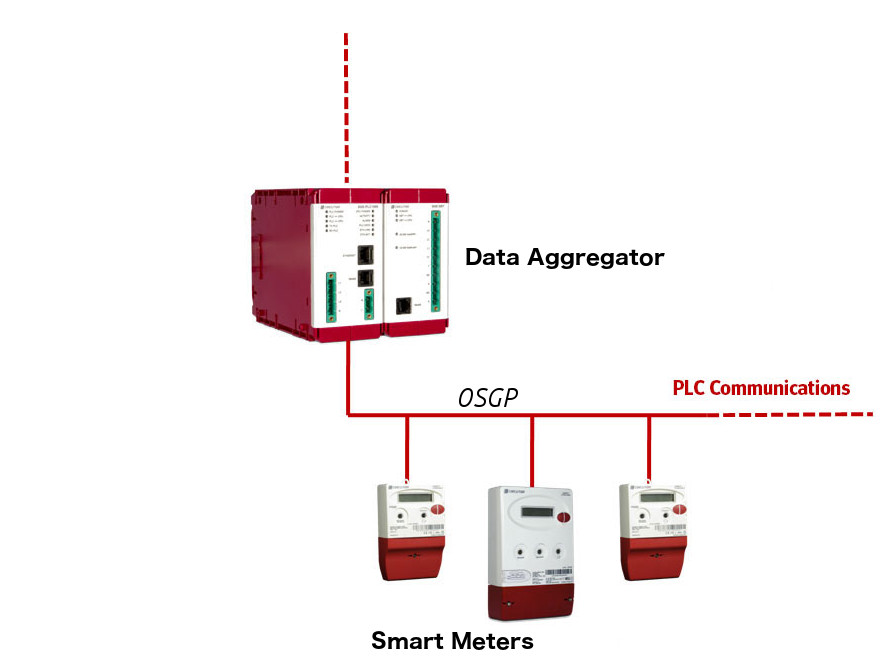
\includegraphics[scale=0.3,cfbox=blue_slides 1pt 0pt]{imgs/aggregator.jpg}
	\end{figure}
\end{frame}

\begin{frame}{Principali vulnerabilità delle Smart Grid: Open Smart Grid Protocol}
	\begin{itemize}[<+- | alert@+>]
		\item Sviluppato da European Telecommunications Standards Institute (ETSI), 2011
		\item Comunicazione su Powerline tra Data Concentrator (Aggregatore) e Smart meter
		\begin{itemize} 
			\item Protocollo Master-Slave: Master (Aggregatore) - Slave (Smart Meter)
			\item Ogni Aggregatore ha una zona di competenza a cui afferisce un certo numero di Smart Meter
		\end{itemize}
	\end{itemize}
	\begin{figure}[h] 
		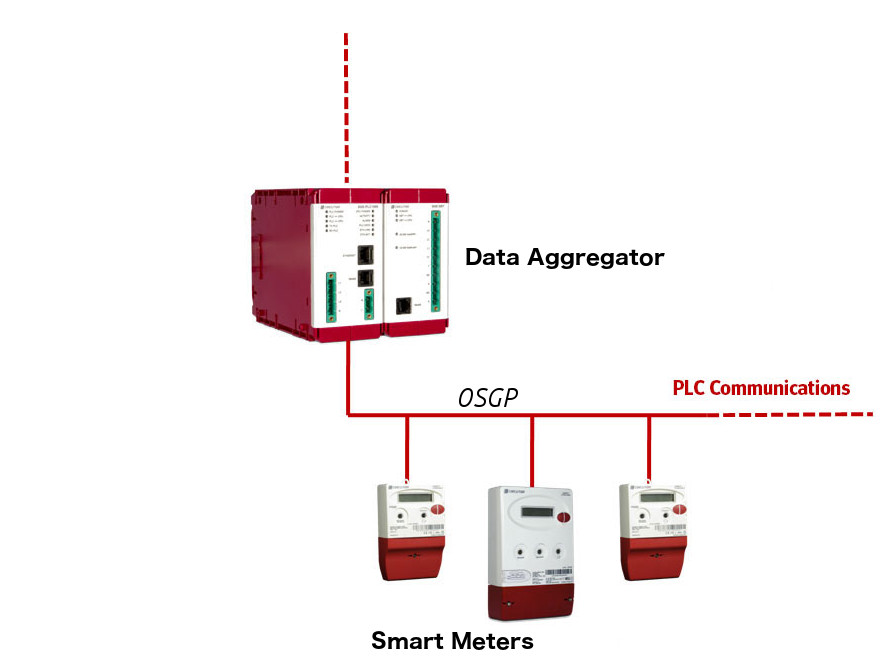
\includegraphics[scale=0.15,cfbox=blue_slides 1pt 0pt]{imgs/aggregator.jpg}
	\end{figure}
\end{frame}

\begin{frame}{Principali vulnerabilità delle Smart Grid: Open Smart Grid Protocol}
	\begin{itemize}[<+- | alert@+>]
		\item Fornisce meccanismi per proteggere la \emph{privacy} dei clienti
		\begin{itemize}[<+- | alert@+>]
			\item Restringendo l'accesso ai dati e cifrandoli evitando accessi non autorizzati
		\end{itemize}
		\item Costruito sullo stack protocollare ISO/IEC 14908-1
		\begin{itemize}[<+- | alert@+>]
			\item Fornisce servizi di autenticazione ma non garantisce \emph{confidentiality} dei dati
		\end{itemize}
		\item Migliora la sicurezza aggiungendo un proprio \emph{security layer}
		%che fornisce autenticazione e confidenzialità
	\end{itemize}
	\begin{figure}[h] 
		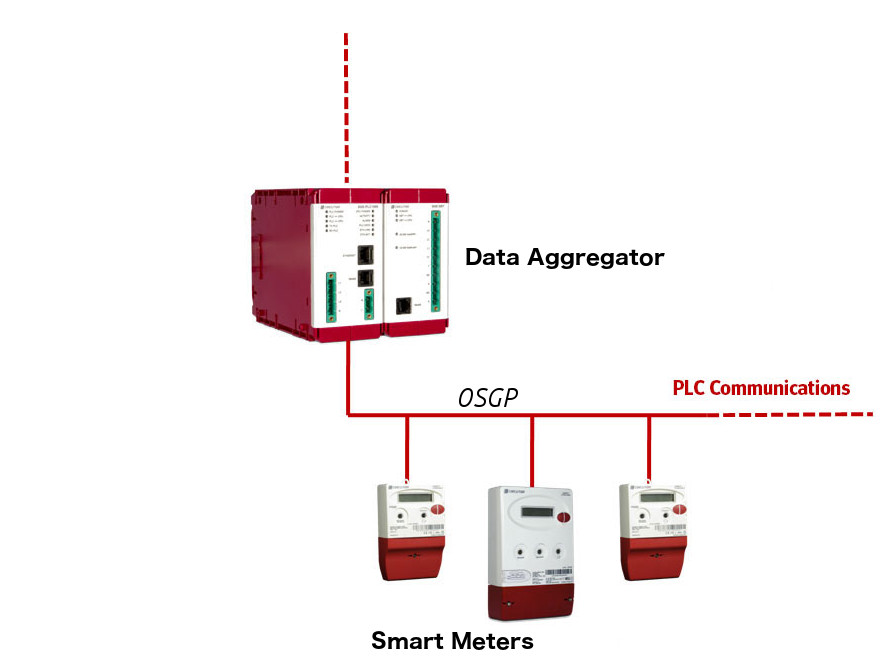
\includegraphics[scale=0.15,cfbox=blue_slides 1pt 0pt]{imgs/aggregator.jpg}
	\end{figure}
\end{frame}

\begin{frame}{Principali vulnerabilità delle Smart Grid: Open Smart Grid Protocol}
	\textbf{Fasi del protocollo OSGP}
	\begin{itemize}
		\item Setup
		\item Communication with Authenticated Encryption
	\end{itemize}
\end{frame}

\begin{frame}{Principali vulnerabilità delle Smart Grid: Open Smart Grid Protocol}
	\textbf{Fasi del protocollo OSGP}
	\begin{itemize}
		\alert<1>{\item Setup}
		\item Communication with Authenticated Encryption
	\end{itemize}
\end{frame}

\begin{frame}{Principali vulnerabilità delle Smart Grid: OSGP - Setup}
	\begin{itemize}[<+- | alert@+>]
		\item Processo di produzione del device OSGP
		\begin{itemize}
			\item Il dispositivo è configurato con una Open Media Access Key (OMAK) univoca a 96 bit
			%chiave principale/di riferimento del dispositivo
		\end{itemize}
		\item La chiave OMAK del device è consegnata alla società di servizi su supporto di memorizzazione
		\item La società di servizi provvede a dotare il Data Concentrator della chiave OMAK del dispositivo afferente alla zona di competenza
	\end{itemize}
\end{frame}
\begin{frame}{Principali vulnerabilità delle Smart Grid: OSGP - Setup}
	\begin{itemize}[<+- | alert@+>]
		\item Il Data Concentrator è in grado di rilevare ogni dispositivo a lui afferente grazie ad un processo di discovery
		\item Il Data Concentrator invia una Shared Key relativa alla sua zona di competenza ad ogni nuovo dispositivo scoperto
		\begin{itemize}
			\item Comunicazione cifrata utilizzando la OMAK del dispositivo
		\end{itemize}
		\item Ogni dispositivo rimpiazza la sua OMAK originaria con la Shared Key ricevuta
	\end{itemize}
\end{frame}
\begin{frame}{Principali vulnerabilità delle Smart Grid: Open Smart Grid Protocol}
	\textbf{Fasi del protocollo OSGP}
	\begin{itemize}
		\item Setup
		\alert<1>{\item Communication with Authenticated Encryption}
	\end{itemize}
\end{frame}

\begin{frame}{Principali vulnerabilità delle Smart Grid: OSGP - Communication with Authenticated Encryption}
	\begin{itemize}[<+- | alert@+>]
		\item Comunicazione iniziata dal Data Concentrator (Master)
		\item Data Concentrator invia messaggio di richiesta allo Smart Meter (Slave)
		\item Smart Meter decifra il messaggio, ne verifica l'autenticità e invia la risposta
		\item Richiesta e risposta cifrate con Shared Key
	\end{itemize}
\end{frame}

\begin{frame}{Principali vulnerabilità delle Smart Grid: OSGP - Authenticated Encryption Scheme}
	\textbf{Schema di cifratura}
	\begin{figure}[h] 
		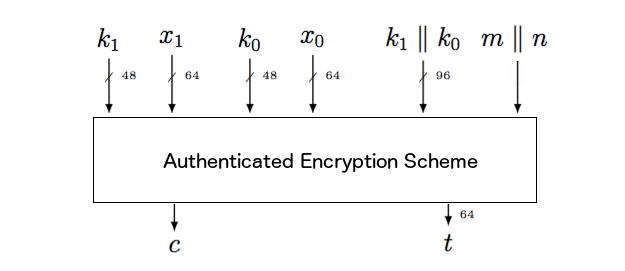
\includegraphics[scale=0.4,cfbox=blue_slides 1pt 0pt]{imgs/c_scheme.png}
	\end{figure}
\end{frame}

\begin{frame}{Principali vulnerabilità delle Smart Grid: OSGP - Authenticated Encryption Scheme}
	\textbf{Parametri di input dello schema di cifratura}
	\begin{itemize}
		\item Costanti
		\begin{itemize}
			\item $x_0 = \{${\tt 81, 3F, 52, 9A, 7B, E3, 89, BA}$\}$, 64 bit
			\item $x_1 = \{${\tt 72, B0, 91, 8D, 44, 05, AA, 57}$\}$, 64 bit
		\end{itemize}
		\pause
		\item Shared Key $k = k_1 \| k_0$
		\begin{itemize}
			\item $k$, 96 bit
			\item $k_1$, 48 bit
			\item $k_0$, 48 bit
		\end{itemize}
	\end{itemize}
\end{frame}

\begin{frame}{Principali vulnerabilità delle Smart Grid: OSGP - Authenticated Encryption Scheme}
	\textbf{Parametri di input dello schema di cifratura}
	\begin{itemize}[<+- | alert@+>]
		\item Messaggio $m$
		\item Sequence number $n$
		\begin{itemize}
			\item Generato in maniera casuale al primo avvio del device
			\item Incrementato dopo ogni messaggio scambiato
			\item Inviato insieme al messaggio
			%\item Utilizzato nella funzione OMADigest
			\item Usato dal ricevitore per verificare la validità del messaggio
			\begin{itemize}
				\item Messaggio valido se $n \in [n-1, n+8]$
				\item In caso contrario, il ricevitore invia messaggio cifrato contenente il sequence number corrente $n$
			\end{itemize}
		\end{itemize}
	\end{itemize}
\end{frame}

\begin{frame}{Principali vulnerabilità delle Smart Grid: OSGP - Authenticated Encryption Scheme}
	\textbf{Parametri di output dello schema di cifratura}
	\begin{itemize}
		\item Tag di autenticazione $t$% \gets OMADigest(k_1\|k_0,\,m\|n)$, 64 bit
		\item Ciphertext $c$% \gets RC4(k^{\prime} \oplus 0^{64}\|t,\,m\|n)$
	\end{itemize}
\end{frame}

\begin{frame}{Principali vulnerabilità delle Smart Grid: OSGP - Authenticated Encryption Scheme}
	\textbf{Building Blocks dello schema di cifratura autenticata}
	\begin{itemize}
		\item Protocollo EN14908
		\item Funzione OMADigest
		\item Algoritmo di cifratura RC4
	\end{itemize}
\end{frame}

\begin{frame}{Principali vulnerabilità delle Smart Grid: OSGP - Authenticated Encryption Scheme}
	\textbf{Building Blocks dello schema di cifratura autenticata}
	\begin{itemize}
		\alert<1>{\item Protocollo EN14908}
		\item Funzione OMADigest
		\item Algoritmo di cifratura RC4
	\end{itemize}
\end{frame}

\begin{frame}{Principali vulnerabilità delle Smart Grid: OSGP - Authenticated Encryption Scheme}
	\textbf{Protocollo EN14908}\\
	Setup iniziale con valore scelto in maniera casuale
	\begin{figure}[h] 
		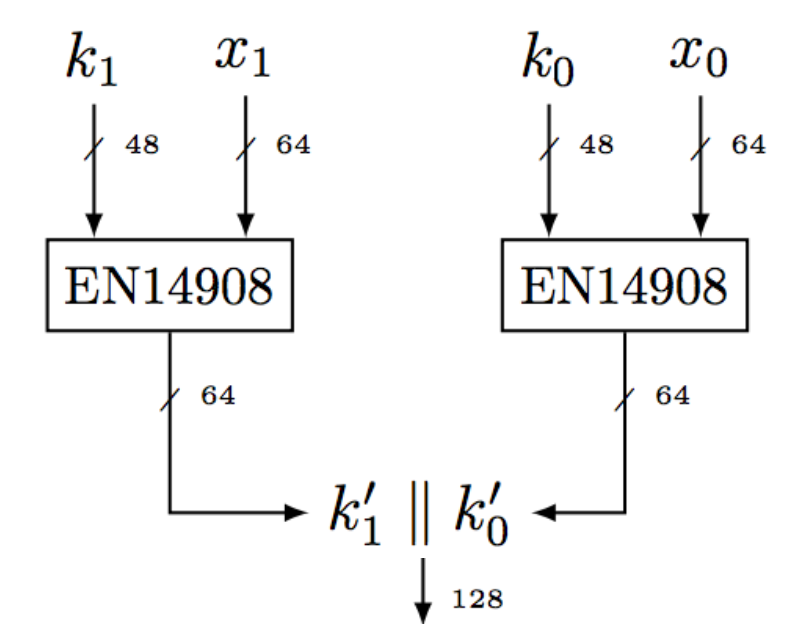
\includegraphics[scale=0.3,cfbox=blue_slides 1pt 0pt]{imgs/EN14908.png}
	\end{figure}
	Base Encryption Key (BEK) $k^{\prime} = k_1^{\prime} \| k_0^{\prime}$
		\begin{itemize}
			\item $k^{\prime}$, 128 bit
			\item $k_1^{\prime} \gets EN14908(k_1,\,x_1)$, 64 bit
			\item $k_0^{\prime} \gets EN14908(k_0,\,x_0)$, 64 bit
		\end{itemize}
\end{frame}

\begin{frame}{Principali vulnerabilità delle Smart Grid: OSGP - Authenticated Encryption Scheme}
	\textbf{Building Blocks dello schema di cifratura autenticata}
	\begin{itemize}
		\item Protocollo EN14908
		\alert<1>{\item Funzione OMADigest}
		\item Algoritmo di cifratura RC4
	\end{itemize}
\end{frame}

\begin{frame}{Principali vulnerabilità delle Smart Grid: OSGP - Authenticated Encryption Scheme}
	\textbf{Funzione OMADigest}
	\begin{figure}[h] 
		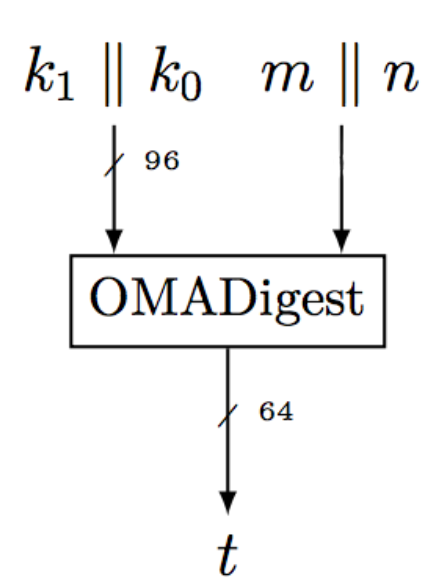
\includegraphics[scale=0.4,cfbox=blue_slides 1pt 0pt]{imgs/OMADigest.png}
	\end{figure}
	\begin{itemize}
		\item Messaggio $m$
		\item Sequence number $n$
		\item Shared Key $k = k_1 \| k_0$
	\end{itemize}
\end{frame}

\begin{frame}{Principali vulnerabilità delle Smart Grid: OSGP - Authenticated Encryption Scheme}
	\textbf{Building Blocks dello schema di cifratura autenticata}
	\begin{itemize}
		\item Protocollo EN14908
		\item Funzione OMADigest
		\alert<1>{\item Algoritmo di cifratura RC4}
	\end{itemize}
\end{frame}

\begin{frame}{Principali vulnerabilità delle Smart Grid: OSGP - Authenticated Encryption Scheme}
	\textbf{Algoritmo di cifratura RC4}
	\begin{itemize}[<+- | alert@+>]
		\item Stream cipher RC4 - Ron Rivest, 1987 (mai pubblicato uff.)
		\begin{itemize}
			\item Periodicità nei primi 256 byte
			\item Forte correlazione fra chiave e keystream (\textit{Breaking 104 bit WEP in less than 60 seconds})
		\end{itemize}
	\end{itemize}
\end{frame}


%\begin{frame}{Principali vulnerabilità delle Smart Grid: OSGP - Authentication}
%	\begin{itemize}[<+- | alert@+>]
%		\item Data concentrator utilizza autenticazione basata su digest a livello applicativo per autenticare messaggi tra i dispositivi
%		\item Viene aggiunto ai messaggi un \emph{sequence number} e se ne effettua il digest, evitando così \emph{replay attack}
%		\item Ogni device sceglie un sequence number $N$ ed accetta solo messaggi aventi sequence number compreso tra $N-1$ e $N+8$
%		% per i restanti manda una response NACK contenente il messaggio "invalid sequence number" seguita dal sequence number desiderato -> il data concentrator deve usare tale numero
%		\item Tutti i dati dei device sono protetti dall’autenticazione basata su digest al livello applicativo sia per operazioni di lettura che di scrittura
%		%include: Configurazione di un dispositivo OSGP, Fatturazioni e profili di carico OSGP, Richieste di cancellazione del carico, Time setting
%
%	\end{itemize}
%\end{frame}

%\begin{frame}{Principali vulnerabilità delle Smart Grid: OSGP - Authentication}
%	\textbf{Request}\newline
%		Formato
%		\begin{figure}[t]
%		
\includegraphics[scale=0.35,cfbox=blue_slides 1pt 0pt]{imgs/req1.png}
%		\end{figure}
%		\pause
%		Digest con OMAK su
%		\begin{figure}[t]
%			
\includegraphics[scale=0.35,cfbox=blue_slides 1pt 0pt]{imgs/req2.png}
%		\end{figure}
%\end{frame}
%
%\begin{frame}{Principali vulnerabilità delle Smart Grid: OSGP - Authentication}
%	\textbf{Response}\newline
%		Formato
%		\begin{figure}[t]
%			
\includegraphics[scale=0.35,cfbox=blue_slides 1pt 0pt]{imgs/res1.png}
%		\end{figure}
%		\pause
%		Digest con OMAK su
%		\begin{figure}[t]
%			
\includegraphics[scale=0.28,cfbox=blue_slides 1pt 0pt]{imgs/res2.png}
%		\end{figure}
%\end{frame}

% Subnet e Node si riferiscono sempre a subnet/node del target della richiesta. Stesso indirizzo in entrambe le direzioni. 
% Request e Sequence fanno riferimento sempre ai valori nel messaggio di richiesta originale.

\begin{frame}{Principali vulnerabilità delle Smart Grid: OSGP - Authenticated Encryption Scheme}
	\begin{figure}[t]
		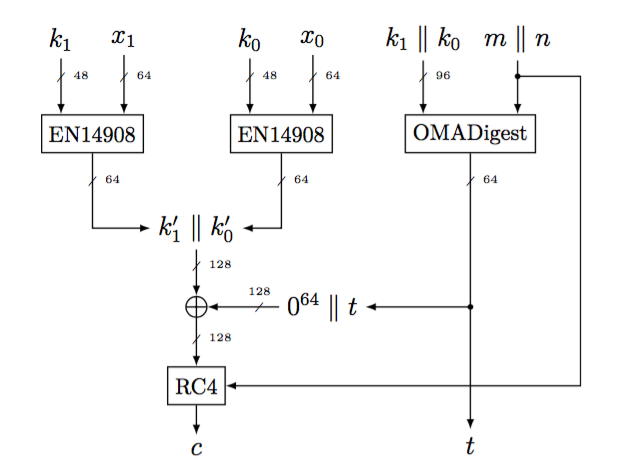
\includegraphics[scale=0.35,cfbox=blue_slides 1pt 0pt]{imgs/osgp.png}
	\end{figure}
	{$t \gets OMADigest(k_1\|k_0,\,m\|n)$, 64 bit}\\
	{$c \gets RC4(k^{\prime} \oplus 0^{64}\|t,\,m\|n)$}
%	\only<1>{Costante $x_0 = \{${\tt 81, 3F, 52, 9A, 7B, E3, 89, BA}$\}$}
%	\only<2>{Costante $x_1 = \{${\tt 72, B0, 91, 8D, 44, 05, AA, 57}$\}$}
%	\only<3>{Open Media Access Key (OMAK) univoca per dispositivo: $k = k_1 \| k_0$}
%	\only<4>{$m$: messaggio}
%	\only<5>{$n$: numero di sequenza}
%	\only<6>{$t$: tag di autenticazione}
%	\only<7>{Base Encryption Key (BEK) $k^\prime = k^{\prime}_{1} \| k^{\prime}_{0}$}
%	\only<8>{$c$: ciphertex}
\end{frame}

%\begin{frame}{Principali vulnerabilità delle Smart Grid: Analisi di OSGP}
%	\textbf{Problemi legati alla sicurezza di OSGP}	
%	\begin{itemize}[<+- | alert@+>]
%		\item OSGP utilizza RC4
%		\begin{itemize}
%			\item L'algoritmo RC4 soggetto ad attacchi di \emph{statistical key recovery} e \emph{plaintext key recovery}
%		\end{itemize}			
%		\item Esiste un algoritmo in grado di invertire la funzione OMADigest
%		\item Chiavi di sessione derivate dalla Shared Key
%			\begin{itemize}
%				\item Determinati attacchi permettono di recuperare la Shared Key
%			\end{itemize}
%	\end{itemize}	
%\end{frame}

\begin{frame}{Principali vulnerabilità delle Smart Grid: sommario}
	\begin{itemize}
		\item Security Testing
		\item Open Smart Grid Protocol
		\alert<1>{\item False Data Injection}
		\item Disconnect Attack
		\item Jamming
	\end{itemize}
\end{frame}

\begin{frame}{Principali vulnerabilità delle Smart Grid: False Data Injection}
	\begin{itemize}[<+- | alert@+>]
		\item Scambio informazioni stato
		\item Stima dello stato $\rightarrow$ Modello \textit{real-time}
		\item Manomettere le misure
		\begin{itemize}
			\item Frode
			\item Sovraccaricare l'infrastruttura
			\item Manipolare prezzi di mercato
		\end{itemize}
		\item \textit{Bad Data Injection}
		\begin{itemize}
			\item Rilevabile
		\end{itemize}
		\item \textit{Stealth Bad Data Injection}
		\begin{itemize}
			\item Non rilevabile
			\item Necessaria conoscenza della topologia
			\item Possibile inferire i parametri legati alla topologia
			\begin{itemize}
				\item \textit{Linear Independent Component Analysis}
			\end{itemize}
		\end{itemize}
	\end{itemize}
\end{frame}
% opzionale %%%%%%%%%%%%%%%%%%%%%%%%%%%%%%%%%%%%%%%%%%%%%%%%%%%%%%%%%%%%%%%%%%%%%
\begin{frame}{Principali vulnerabilità delle Smart Grid: attacchi e contromisure}
\textbf{Modello Matematico}
	\begin{block}{Vettore delle misurazioni} % vorrei mettere tipo l'alert
		$\textbf{z} = \textbf{h(x)} + \textbf{e}$
		\begin{itemize}
			\item $\textbf{h(x)}$: relazione non lineare tra le misure $\textbf{z}$ e lo stato del sistema $\textbf{x}$
			\item $\textbf{e} = [e_1, \ldots, e_m]^T$, rumore Gaussiano delle misure
		\end{itemize}
	\end{block}
	\pause
	\begin{block}{Modello di approssimazione lineare della misura di corrente}
		Misura sotto Operazioni Normali: $\textbf{z} =  \textbf{Hx} + \textbf{e}$
		\begin{itemize}
			\item Vettore di stato stimato: $\widehat{\textbf{x}} = (\textbf{H}^T\sum_e^{-1}\textbf{H})-1\textbf{H}^T\sum_e^{-1}\textbf{z}$
			\item $\textbf{H} \in {\rm I\!R}$, definito come
			\begin{itemize}
				\item $\textbf{H}=\frac{\partial\textbf{h(x)}}{\partial\textbf{x}}|_{x=0}$
			\end{itemize}
			\item Matrice di covarianza $\Sigma_e$
		\end{itemize}
	\end{block}
\end{frame}

\begin{frame}{Principali vulnerabilità delle Smart Grid: attacchi e contromisure}
	\textbf{Modello Matematico}
	\begin{itemize}
	\item Bad Data Injection
	\begin{itemize}
		\item Misura sotto attacco non stealth: $\textbf{z}^\prime = \textbf{H}(\textbf{x}) + \textbf{b} + e$
		\item Vettore residuo: $\textbf{r} = \textbf{z} - \textbf{H}\widehat{\textbf{x}}$
		\item Rilevamento bad data: $max_i(|\textbf{r}_i|/\sqrt{cov(\textbf{r})}) \geq \gamma$
	\end{itemize}
	\item Stealth Bad Data Injection
	\begin{itemize}
		\item Misura sotto attacco stealth: $\textbf{z}^\prime = \textbf{H}(\textbf{x} + \delta\textbf{x}) + e$
		\item Non rilevabile usando meccanismi a soglia
	\end{itemize}
\end{itemize}
\let\thefootnote\relax\footnote{$\textbf{H}(\textbf{x})$ e $\textbf{H}(\textbf{x} + \delta\textbf{x})$ sono prodotti $matrice \times vettore$}
\end{frame}
%%%%%%%%%%%%%%%%%%%%%%%%%%%%%%%%%%%%%%%%%%%%%%%%%%%%%%%%%%%%%%%%%%%%%%%%%%%%%%%%%

\begin{frame}{Principali vulnerabilità delle Smart Grid: sommario}
	\begin{itemize}
		\item Security Testing
		\item Open Smart Grid Protocol
		\item False Data Injection
		\alert<1>{\item Disconnect Attack}
		\item Jamming
	\end{itemize}
\end{frame}

\begin{frame}{Principali vulnerabilità delle Smart Grid: Disconnect Attack}
	\begin{itemize}[<+- | alert@+>]
		\item Remote Connect Disconnect (RCD)
		\item Attacco RCD $\rightarrow$ Blackout/Danni alla rete
		\item Difesa: ritardi casuali nell'esecuzione dei comandi RCD
		\begin{itemize}
			\item Prevenire rapidi cambiamenti del carico elettrico
			\item Tempo per rilevare e fermare un attacco in corso
		\end{itemize}
	\end{itemize}
\end{frame}

\begin{frame}{Principali vulnerabilità delle Smart Grid: sommario}
	\begin{itemize}
		\item Security Testing
		\item Open Smart Grid Protocol
		\item False Data Injection
		\item Disconnect Attack
		\alert<1>{\item Jamming}
	\end{itemize}
\end{frame}

\begin{frame}{Principali vulnerabilità delle Smart Grid: Jamming}
	\begin{block}{}
	Strategia d'attacco utilizzata per la manipolazione del mercato elettrico
	\end{block}
	\pause
	\begin{block}{Assunzione}
	Si utilizza un sistema di comunicazione wireless, come \textbf{\color{blue_slides}WiMAX}, per effettuare il broadcast delle informazioni relative ai prezzi
	\end{block}
\end{frame}

\begin{frame}{Principali vulnerabilità delle Smart Grid: Jamming}
	\textbf{Attacco}\\
	{\small [Li, Husheng, and Zhu Han. ``Manipulating the electricity power market via jamming the price signaling in smart grid.'' \emph{GLOBECOM Workshops (GC Wkshps), 2011 IEEE}. IEEE, 2011.]}
	\begin{enumerate}[<+- | alert@+>]
		\item L'attaccante fa Jamming in un'area molto popolata
		\item L'utente rimane a conoscenza del vecchio prezzo della corrente
		\item L'attaccante monitora il mercato elettrico
		\item Quando il prezzo cambia significativamente, si smette di fare Jamming
		\item Ogni utente adatta il proprio consumo energetico in base al nuovo prezzo
		%se il nuovo prezzo è superiore, l'utente diminuisce i consumi, facendo calare il prezzo con p alta. se il nuovo prezzo è più piccolo, l'utente incrementa i consumi, aumentando con alta probabilità il prezzo.
		\item L'attaccante può avere profitti da questa manipolazione del mercato
		%è in grado di predire come si comporteranno gli utenti alla ricezione del nuovo prezzo e quindi sono in grado di cambiare il prezzo della corrente quando e come vogliono.
	\end{enumerate}
\end{frame}

\begin{frame}{Principali vulnerabilità delle Smart Grid: Jamming}
	\begin{block}{Contromisure}
		Evitare di modificare il consumo di energia in maniera simultanea.\newline
		\textbf{\color{blue_slides}IDEA: si utilizza uno schema di \emph{backoff}} 
	\end{block}
	\pause
	\begin{block}{}
	Ogni consumer sceglie un tempo casuale per cambiare la propria power response evitando che l'attaccante possa predire il comportamento dell'utente e quindi capire in che modo varia il prezzo della corrente
		%randomness: perchè i consumi sono in base alle esigenze e tendono a variare da persona a persona
		%utilizzando backoff casuali per evitare collisioni dovute a trasmissioni simultanee
		%schema di backoff casuale: un consumer sceglie un tempo casuale per cambiare la propria power response
		%si diffondono info relative ai cambiamenti in un intervallo di tempo piu ampio cosicchè la randomness del mercato possa contrattaccare i cambiamenti dei jammed user
	\end{block}
\end{frame}

{\renewcommand{\addtocontents}[2]{}
\section*{Grazie per l'attenzione!}}


%\begin{frame}[fragile]
%  \frametitle{mtheme}
%
%  The \textsc{Metropolis} theme is a Beamer theme with minimal visual noise
%  inspired by the \href{https://github.com/hsrmbeamertheme/hsrmbeamertheme}{\textsc{hsrm} Beamer
%  Theme} by Benjamin Weiss.
%
%  Enable the theme by loading
%
%  \begin{verbatim}    \documentclass{beamer}
%    \usetheme{m}\end{verbatim}
%
%  Note, that you have to have Mozilla's \emph{Fira Sans} font and XeTeX
%  installed to enjoy this wonderful typography.
%\end{frame}
%\begin{frame}[fragile]
%  \frametitle{Sections}
%  Sections group slides of the same topic
%
%  \begin{verbatim}    \section{Elements}\end{verbatim}
%
%  for which \textsc{Metropolis} provides a nice progress indicator \ldots
%\end{frame}
%
%\section{Elements}
%
%\begin{frame}[fragile]
%  \frametitle{Typography}
%      \begin{verbatim}The theme provides sensible defaults to
%\emph{emphasize} text, \alert{accent} parts
%or show \textbf{bold} results.\end{verbatim}
%
%  \begin{center}becomes\end{center}
%
%  The theme provides sensible defaults to \emph{emphasize} text,
%  \alert{accent} parts or show \textbf{bold} results.
%\end{frame}
%\begin{frame}{Lists}
%  \begin{columns}[T,onlytextwidth]
%    \column{0.33\textwidth}
%      Items
%      \begin{itemize}
%        \item Milk \item Eggs \item Potatos
%      \end{itemize}
%
%    \column{0.33\textwidth}
%      Enumerations
%      \begin{enumerate}
%        \item First, \item Second and \item Last.
%      \end{enumerate}
%
%    \column{0.33\textwidth}
%      Descriptions
%      \begin{description}
%        \item[PowerPoint] Meeh. \item[Beamer] Yeeeha.
%      \end{description}
%  \end{columns}
%\end{frame}
%\begin{frame}{Animation}
%  \begin{itemize}[<+- | alert@+>]
%    \item \alert<4>{This is\only<4>{ really} important}
%    \item Now this
%    \item And now this
%  \end{itemize}
%\end{frame}
%\begin{frame}{Figures}
%  \begin{figure}
%    \newcounter{density}
%    \setcounter{density}{20}
%    \begin{tikzpicture}
%      \def\couleur{alerted text.fg}
%      \path[coordinate] (0,0)  coordinate(A)
%                  ++( 90:5cm) coordinate(B)
%                  ++(0:5cm) coordinate(C)
%                  ++(-90:5cm) coordinate(D);
%      \draw[fill=\couleur!\thedensity] (A) -- (B) -- (C) --(D) -- cycle;
%      \foreach \x in {1,...,40}{%
%          \pgfmathsetcounter{density}{\thedensity+20}
%          \setcounter{density}{\thedensity}
%          \path[coordinate] coordinate(X) at (A){};
%          \path[coordinate] (A) -- (B) coordinate[pos=.10](A)
%                              -- (C) coordinate[pos=.10](B)
%                              -- (D) coordinate[pos=.10](C)
%                              -- (X) coordinate[pos=.10](D);
%          \draw[fill=\couleur!\thedensity] (A)--(B)--(C)-- (D) -- cycle;
%      }
%    \end{tikzpicture}
%    \caption{Rotated square from
%    \href{http://www.texample.net/tikz/examples/rotated-polygons/}{texample.net}.}
%  \end{figure}
%\end{frame}
%\begin{frame}{Tables}
%  \begin{table}
%    \caption{Largest cities in the world (source: Wikipedia)}
%    \begin{tabular}{lr}
%      \toprule
%      City & Population\\
%      \midrule
%      Mexico City & 20,116,842\\
%      Shanghai & 19,210,000\\
%      Peking & 15,796,450\\
%      Istanbul & 14,160,467\\
%      \bottomrule
%    \end{tabular}
%  \end{table}
%\end{frame}
%\begin{frame}{Blocks}
%  Three different block environments are pre-defined and may be styled with an
%  optional background color.
%
%  \begin{columns}[T,onlytextwidth]
%    \column{0.5\textwidth}
%      \begin{block}{Default}
%        Block content.
%      \end{block}
%
%      \begin{alertblock}{Alert}
%        Block content.
%      \end{alertblock}
%
%      \begin{exampleblock}{Example}
%        Block content.
%      \end{exampleblock}
%
%    \column{0.5\textwidth}
%
%      \metroset{block=fill}
%
%      \begin{block}{Default}
%        Block content.
%      \end{block}
%
%      \begin{alertblock}{Alert}
%        Block content.
%      \end{alertblock}
%
%      \begin{exampleblock}{Example}
%        Block content.
%      \end{exampleblock}
%
%  \end{columns}
%\end{frame}
%\begin{frame}{Math}
%  \begin{equation*}
%    e = \lim_{n\to \infty} \left(1 + \frac{1}{n}\right)^n
%  \end{equation*}
%\end{frame}
%\begin{frame}{Line plots}
%  \begin{figure}
%    \begin{tikzpicture}
%      \begin{axis}[
%        mlineplot,
%        width=0.9\textwidth,
%        height=6cm,
%      ]
%
%        \addplot {sin(deg(x))};
%        \addplot+[samples=100] {sin(deg(2*x))};
%
%      \end{axis}
%    \end{tikzpicture}
%  \end{figure}
%\end{frame}
%\begin{frame}{Bar charts}
%  \begin{figure}
%    \begin{tikzpicture}
%      \begin{axis}[
%        mbarplot,
%        xlabel={Foo},
%        ylabel={Bar},
%        width=0.9\textwidth,
%        height=6cm,
%      ]
%
%      \addplot plot coordinates {(1, 20) (2, 25) (3, 22.4) (4, 12.4)};
%      \addplot plot coordinates {(1, 18) (2, 24) (3, 23.5) (4, 13.2)};
%      \addplot plot coordinates {(1, 10) (2, 19) (3, 25) (4, 15.2)};
%
%      \legend{lorem, ipsum, dolor}
%
%      \end{axis}
%    \end{tikzpicture}
%  \end{figure}
%\end{frame}
%\begin{frame}{Quotes}
%  \begin{quote}
%    Veni, Vidi, Vici
%  \end{quote}
%\end{frame}
%
%\begin{frame}{References}
%  Some references to showcase [allowframebreaks] \cite{knuth92,ConcreteMath,Simpson,Er01,greenwade93}
%\end{frame}
%
%\section{Conclusion}
%
%\begin{frame}{Summary}
%
%  Get the source of this theme and the demo presentation from
%
%  \begin{center}\url{github.com/matze/mtheme}\end{center}
%
%  The theme \emph{itself} is licensed under a
%  \href{http://creativecommons.org/licenses/by-sa/4.0/}{Creative Commons
%  Attribution-ShareAlike 4.0 International License}.
%
%  \begin{center}\ccbysa\end{center}
%
%\end{frame}
%
%\plain{Questions?}
%
%\begin{frame}[allowframebreaks]
%
%  \frametitle{References}
%
%  \bibliography{demo}
%  \bibliographystyle{abbrv}
%
%\end{frame}

\end{document}
